\documentclass[]{beamer}
\usepackage{CJKutf8}
\usepackage[utf8]{inputenc}
\usepackage[T1]{fontenc}
\usepackage{listings}
\usetheme{Gipsalab}
\setbeamertemplate{navigation symbols}{}
%============================================================================
\author[G. Becq]{Guillaume Becq}
\title[Introduction à Python]{Introduction au langage de programmation Python}
\subtitle{{\footnotesize Une pas si courte introduction à Python comme alternative à Matlab pour réaliser des calculs scientifiques ou d'autres applications.}}
\date{\today}
%============================================================================
%===============================================================================
% General 
%_______________________________________________________________________________
\DeclareRobustCommand{\myFrame}[3]{%
\begin{frame}
\frametitle{#1}
\framesubtitle{#2}
#3
\end{frame}}
%_______________________________________________________________________________
%_______________________________________________________________________________
\newcommand{\myFrameInput}[3]{%
\frametitle{#1}
\framesubtitle{#2}
\input{#3}
\end{frame}}
%_______________________________________________________________________________
%_______________________________________________________________________________
\newcommand{\myFig}[2]{\includegraphics[#1]{#2}}
\newcommand{\hide}[1]{}
\newcommand{\urlPython}{\url{www.python.org}}
\newcommand{\comment}[1]{}
%_______________________________________________________________________________

%===============================================================================
%===============================================================================
% Beamer
%_______________________________________________________________________________
% frame CLR 
% up Center down Left + Right 
%  [  ]
% [ ][ ] ; 
% \frameCLR{12cm}{3cm}{partUp}{partDownLeft}{partDownRight}
\newcommand{\frameCLR}[5]{\begin{center}#3\end{center}% 
\begin{minipage}[c]{#1}#4\end{minipage}\hfill%
\begin{minipage}[c]{#2}#5\end{minipage}}
%_______________________________________________________________________________
%_______________________________________________________________________________
% frame CCC
% three centered parts: up, middle, down
%   []
%  [  ]
%   []
% \frameCCC{partUp}{partMiddle}{partDown}
\newcommand{\frameCCC}[3]{\begin{center}#1\end{center}% 
\begin{center}#2\end{center}% 
\begin{center}#3\end{center}}
%_______________________________________________________________________________
%_______________________________________________________________________________
% frame CC
% two centered parts: up, down
%   []
%  [  ]
% \frameCC{partUp}{partDown}
\newcommand{\frameCC}[2]{\begin{center}#1\end{center}% 
\begin{center}#2\end{center}}
%_______________________________________________________________________________
%_______________________________________________________________________________
% frame C
% one centered part:
%  [  ]
% \frameC{part}
\newcommand{\frameC}[1]{\begin{center}#1\end{center}}
%_______________________________________________________________________________
%_______________________________________________________________________________
% frame LR
% two parts: left + right 
% [   ][ ]  
% \frameLR{12cm}{3cm}{partLeft}{partRight}
\newcommand{\frameLR}[4]{\begin{minipage}[c]{#1}#3\end{minipage}\hfill% 
\begin{minipage}[c]{#2}#4\end{minipage}}
%_______________________________________________________________________________
%_______________________________________________________________________________
\newcommand{\framePlan}{%
\begin{frame}\tableofcontents[subsectionstyle=hide]\end{frame}}
%_______________________________________________________________________________
%_______________________________________________________________________________
\newcommand{\framePlanCurrentSection}{%
\begin{frame}\frametitle{Outline}%
\tableofcontents[currentsection, subsectionstyle=hide]\end{frame}}
%_______________________________________________________________________________
%===============================================================================
%===============================================================================
% Colors
%===============================================================================
%_______________________________________________________________________________
\definecolor{pythonBackground}{rgb}{0.8,1,1}
%_______________________________________________________________________________
%_______________________________________________________________________________
\definecolor{matlabBackground}{rgb}{1,0.8,0.8}
%_______________________________________________________________________________
%===============================================================================
%===============================================================================
% listings
%===============================================================================
%_______________________________________________________________________________
\lstdefinestyle{myPython}{language=python, keywordstyle=\color{blue}, commentstyle=\color{red}, basicstyle=\tiny \ttfamily, stringstyle=\color{magenta}\ttfamily, backgroundcolor=\color{pythonBackground}, showstringspaces=false, texcl=true, escapechar=£}
%_______________________________________________________________________________
%_______________________________________________________________________________
\lstdefinestyle{myPythonConsole}{language=python, keywordstyle=\color{blue}, commentstyle=\color{red}, basicstyle=\tiny \ttfamily, stringstyle=\color{magenta} \ttfamily, backgroundcolor=\color{pythonBackground}, texcl=true, escapechar=£}
%_______________________________________________________________________________
%_______________________________________________________________________________
\lstdefinestyle{myMatlab}{language=matlab, keywordstyle=\color{blue}, commentstyle=\color{red}, basicstyle=\tiny \ttfamily, showstringspaces=false,  stringstyle=\color{magenta} \ttfamily, backgroundcolor=\color{matlabBackground}, escapechar=£}
%_______________________________________________________________________________
%_______________________________________________________________________________
\lstdefinestyle{myShell}{language=bash, basicstyle=\tiny \ttfamily, backgroundcolor=\color{pythonBackground}, escapechar=£}
%_______________________________________________________________________________
%_______________________________________________________________________________
\lstnewenvironment{python}{\lstset{style=myPython}}{}
%_______________________________________________________________________________
%_______________________________________________________________________________
\lstnewenvironment{shell}{\lstset{style=myShell}}{}
%_______________________________________________________________________________
%_______________________________________________________________________________
\lstnewenvironment{pythonConsole}{\lstset{style=myPythonConsole}}{}
%_______________________________________________________________________________
%_______________________________________________________________________________
\newcommand{\lstinputpython}[1]{\lstinputlisting[style=myPython]{#1}}
%_______________________________________________________________________________
%_______________________________________________________________________________
\lstnewenvironment{matlab}{\lstset{style=myMatlab}}{}
%_______________________________________________________________________________
%===============================================================================


\AtBeginSection{\framePlanCurrentSection}
%============================================================================
%============================================================================
\includeonly{%
sec_introduction, 
sec_language, 
sec_scientific, 
sec_environment, 
sec_conclusion, 
sec_appendix, 
}

%============================================================================
\begin{document}
%____________________________________________________________________________
\begin{frame}[plain]
\maketitle
\end{frame}
\framePlan
%===============================================================================
\section{Introduction}
%_______________________________________________________________________________
\subsection{Historique}
%...............................................................................
\begin{frame}[fragile]
\frametitle{Historique}
\framesubtitle{Python}
\frameLR{7cm}{3cm}
{%
\begin{itemize}
\item 1989--1995 : Hollande
\only<2>{%
\small
\begin{itemize}
 \item Centrum voor Wiskunde en Informatica (CWI). 
 \item \emph{Guido von Rossum}, fan des Monty Python, travaille sur : 
 \begin{itemize}
  \item ABC : langage de script, syntaxe et indentation. 
  \item Modula-3 : gestion des exceptions, orienté objet. 
  \item langage C, Unix.
  \item OS distribué Amoeba: accès difficile en shell.
 \end{itemize}
 \item Créée le langage Python :
 \begin{itemize}
  \item 1991/02 : versions 0.9.06 déposée sur un newsgroup de Usenet
  \item 1995 : dépôt de la version 1.2
 \end{itemize}
\end{itemize}}
\item 1995--1999 : USA 
\only<3>{%
\small
\begin{itemize}
 \item Corporation for National Research Initiatives (CNRI), non profit organisation, Reston, USA.
 \item Grail7 : navigateur internet utilisant Tk. 
 \item 1999 : projet \emph{Computer Programming for Everybody} (CP4E) (CNRI, DARPA Defense Advanced Research Projects Agency) :
 \begin{itemize}
  \item Python comme langage d'enseignement de la programmation. 
  \item Création de l'IDLE (Integrated DeveLopment Environment)
 \end{itemize}
 \item 1999 : Python 1.6
\end{itemize}}
\item 1999+ : Worldwide open source
\only<4>{%
\small
\begin{itemize}
 \item BeOpen.com :
 \begin{itemize} 
  \item compatibilité GPL (General Public Licence)
  \item création de la branche pythonLabs
 \end{itemize}
 \item 2000 : Python Software Foundation 
 \begin{itemize} 
  \item Python 2.1 : changement licence, dérivée de Apache Software Foundation (OO, svn, commons plutôt java) (\url{http://www.apache.org}). 
 \end{itemize} 
 \item 2008: Python 3.0 
\end{itemize}}
\end{itemize}
{\tiny sources : \url{http://www.wikipedia.org}, \url{http://www.python.org}}%
}
{%
\only<2>{\myFig{width=2cm}{./fig/MontyPythonFoot.png} \\ \myFig{width=3cm}{./fig/ordi1990.jpg}}%
\only<3>{\myFig{width=3cm}{./fig/grail.png}}%
\only<4>{\myFig{width=3cm}{./fig/python-logo.png}}%
}
\end{frame}
%...............................................................................
%...............................................................................
\begin{frame}
\frametitle{Historique}
\framesubtitle{Guido van Rossum}
\frameLR{7cm}{3cm}{%
\begin{itemize}
 \item Guido van Rossum : 
 \begin{itemize}
  \item 31 janvier 1956 (59 ans)
  \item Développeur néerlandais
  \item 1982 : M. Sc  
  \item Développeur ABC. 
 \end{itemize} 
 \item Créateur Python : \emph{Benevolent Dictator For Life (BDFL)}
 \begin{itemize}
  \item 1991 : Python 0.9.06
  \item 1999 : Grail
 \end{itemize}
 \item 2002 : Prix pour le développement du logiciel libre 2001 décerné par la \emph{Free Software Foundation}
 \item 2005--2012 : Google (python) 
 \item 2013 : Dropbox
\end{itemize}
{\tiny sources : \url{http://www.wikipedia.org}, \url{http://www.python.org}}%
}
{%
\myFig{width=3cm}{./fig/guido.jpg} \\ 
{\tiny 2006, source wikipedia}%
}
\end{frame}

%...............................................................................
%_______________________________________________________________________________
%_______________________________________________________________________________
\subsection{Spécificités}
%...............................................................................
\begin{frame}
\frametitle{Spécificités}
\framesubtitle{}
\url{http://www.python.org/about/}
\begin{itemize}
 \item Fortement typé.  
 \item Objet.
 \item Script, séquentiel, interprété : fichier génère du byte code.
 \item Comparé à Tcl, Perl, Ruby, Scheme, Java.
\end{itemize}
\end{frame}
%...............................................................................
%...............................................................................
\begin{frame}[fragile]
\frametitle{Spécificités}
\framesubtitle{Exemple 1er programme}
Dans le fichier "hello.py" : 
\begin{python}
print("Bonjour monde")
\end{python}

Exécution dans une interface système (terminal, shell) : 
\begin{shell}
~/python/example> python hello.py
Bonjour monde
\end{shell}
\end{frame}
%...............................................................................
%...............................................................................
\begin{frame}[fragile]
\frametitle{Spécificités}
\framesubtitle{Exemple shell scripting}
Exemple copies des fichiers '.txt' et '.tex' du répertoire 'a' vers 'b'.
\lstinputlisting[style=myPython]{./example/shell/shellScript.py}
\end{frame}
%...............................................................................
%_______________________________________________________________________________
%_______________________________________________________________________________
\subsection{Utilisation}
%...............................................................................
\begin{frame}[fragile]
\frametitle{Utilisations}
\framesubtitle{A partir du shell}
\begin{itemize}
\item Fichiers "*.py" contient des scripts et des définitions de fonctions.
Ils sont exécutés dans le shell avec la commande "python". 

Exemple : "python hello.py" 

\item La commande "python" ouvre une console utilisateur (\emph{interpreter}) avec une invite de commande (prompt) caractéristique "> > > "
\end{itemize}

\begin{python}
Enthought Canopy Python 2.7.3 | 64-bit | (default, Jun 14 2013, 18:17:36) 
[GCC 4.2.1 (Apple Inc. build 5666) (dot 3)] on darwin
Type "help", "copyright", "credits" £or£ "license" £for£ more information.
>>> 
\end{python}

\end{frame}
%...............................................................................
%...............................................................................
\begin{frame}[fragile]
\frametitle{Utilisations}
\framesubtitle{Utilisation de l'interpréteur}
\begin{itemize}
\item Association d'une valeur à une variable : a = 'abc'
\item Affichage de la valeur : print()
\item Liste des noms, attributs, fonctions disponibles : dir()
\end{itemize}

\begin{python}
>>> a = "abc"
>>> print(a)
abc
>>> dir()
['__builtins__', '__doc__', '__name__', '__package__', 'a']

>>> dir(a)
['__add__', '__class__', '__contains__', '__delattr__', '__doc__', 
'__eq__', '__format__', '__ge__', '__getattribute__', '__getitem__',
'__getnewargs__', '__getslice__', '__gt__', '__hash__', '__init__', 
'__le__', '__len__', '__lt__', '__mod__', '__mul__', '__ne__', '__new__', 
'__reduce__', '__reduce_ex__', '__repr__', '__rmod__', '__rmul__', 
'__setattr__', '__sizeof__', '__str__', '__subclasshook__', 
'_formatter_field_name_split', '_formatter_parser', 'capitalize', 
'center', 'count', 'decode', 'encode', 'endswith', 'expandtabs', 'find',
'format', 'index', 'isalnum', 'isalpha', 'isdigit', 'islower', 'isspace',
'istitle', 'isupper', 'join', 'ljust', 'lower', 'lstrip', 'partition',
'replace', 'rfind', 'rindex', 'rjust', 'rpartition', 'rsplit', 'rstrip',
'split', 'splitlines', 'startswith', 'strip', 'swapcase', 'title', 
'translate', 'upper', 'zfill']
\end{python}
\end{frame}
%...............................................................................
%...............................................................................
\begin{frame}[fragile]
\frametitle{Utilisations}
\framesubtitle{Utilisation de l'interpréteur}
\begin{itemize}
 \item Besoin d'aide : help()
\end{itemize}
\begin{pythonConsole}
>>> help(a.find)

Help on built-£in£ function find:

find(...)
    S.find(sub [,start [,end]]) -> int
    
    Return the lowest index £in£ S where substring sub £is£ found,
    such that sub £is£ contained within S[start:end].  Optional
    arguments start £and£ end are interpreted as £in£ slice notation.
    
    Return -1 on failure.
(END) 
\end{pythonConsole}
\end{frame}
%...............................................................................
%_______________________________________________________________________________
%_______________________________________________________________________________
\subsection{Site web}
%...............................................................................
\begin{frame}
\frametitle{Site Web}
\framesubtitle{www.python.org}
\frameC{\myFig{width=10cm}{./fig/sitePython.png}}
\end{frame}
%...............................................................................
%_______________________________________________________________________________
%_______________________________________________________________________________
\subsection{Documentation}
%...............................................................................
\begin{frame}
\frametitle{Documentation}
\framesubtitle{Trouver la documentation}
\frameC{\myFig{width=10cm}{./fig/sitePythonDoc.png}}
\end{frame}
%...............................................................................
%...............................................................................
\begin{frame}
\frametitle{Documentation}
\framesubtitle{Lire la documentation - Tutorial}
\frameC{\myFig{width=10cm}{./fig/PDFTutorial.png}}
\end{frame}
%...............................................................................
%...............................................................................
\begin{frame}
\frametitle{Documentation}
\framesubtitle{Lire la documentation - Library reference}
\frameC{\myFig{width=10cm}{./fig/PDFLibrary.png}}
\end{frame}
%...............................................................................
%...............................................................................
\begin{frame}
\frametitle{Documentation}
\framesubtitle{Lire la documentation - Library reference}
\frameC{\myFig{width=10cm}{./fig/PDFLibraryOS.png}}
\end{frame}
%...............................................................................
%...............................................................................
\begin{frame}
\frametitle{Documentation}
\framesubtitle{Lire la documentation - Language reference}
\frameC{\myFig{width=10cm}{./fig/PDFReference.png}%

{\scriptsize\textit{p. ex. grammaire sous forme de Backus-Naur (BNF)}}}
\end{frame}
%...............................................................................
%...............................................................................
\begin{frame}
\frametitle{Python Enhancements Proposals}
\framesubtitle{PEPs}
\frameCC{% 
Propositions et conseils pour l'utilisation et l'amélioration du langage.}
{%
\myFig{width=8cm}{./fig/sitePythonPEPs.png}
}
\end{frame}
%...............................................................................
%_______________________________________________________________________________
%_______________________________________________________________________________
\subsection{Installation}
%...............................................................................
\begin{frame}
\frametitle{Installation}
\framesubtitle{}
\begin{itemize}
 \item Téléchargement sous \urlPython\ pour les OS courants : Windows, Linux, Mac. 
 \item 32 bits vs 64 bits : 
  \begin{itemize}
   \small
   \item Performances vs compatibilités bibliothèques (paquets) 
   \item Problèmes de configuration des compilateurs (gcc).
  \end{itemize}
 \item Autres distributions : Enthought Canopy, pythonXY, Anaconda, WinPython, \dots 
 \item Implémentations alternatives : 
 \begin{itemize}
  \small
  \item Langage identique mais implémentation différentes permet par exemple : d'interfacer du java facilement (Jython), d'être plus performant pour les calculs avec un compilateur JIT (Pypy)\dots
 \end{itemize}
\end{itemize}
\end{frame}
%...............................................................................
%...............................................................................
\begin{frame}
\frametitle{Installation}
\framesubtitle{Python 2.7 vs 3.x}

\begin{itemize}
\item 2.7 : figée.
\item 3.x : présent et futur : 
\begin{itemize}
 \item {\it better Unicode support}
 \item Quelques inconsistences du langage (ex print 'a' vs print('a')).  
 \item Résultats de la division des entiers (1/2 : 2.x, = 0 ; 3.x, = 0.5). 
 \item \dots
\end{itemize}
\item Peut poser des problèmes :
\begin{itemize}
 \item Paquets portées sur 3.x ?
 \item Compatibilité 64 bits ? 
\end{itemize}
\end{itemize}
\end{frame}
%...............................................................................
%_______________________________________________________________________________
%===============================================================================


%===============================================================================
\section{Description du Langage}
%_______________________________________________________________________________
\subsection{Type de données}
%...............................................................................
\begin{frame}
\frametitle{Type de base}
\framesubtitle{}
\begin{itemize}
\item {\bfseries Nombres} : entiers (int, long), réels (float), complex (complex), booléens (bool). 
\item {\bfseries Séquences} : Chaînes de caractères (str), listes (list), tuples (tuple), dictionnaires (dict), ensembles (set)
\end{itemize}
\end{frame}
%...............................................................................
%...............................................................................
\begin{frame}[fragile]
\frametitle{Nombres}
\framesubtitle{Entiers}
\begin{itemize}
 \item Attention à la division entière en 2.7. 
\end{itemize}
\begin{pythonConsole}
>>> a = 1  
>>> b = 2
>>> c = a / b
>>> print(c)
0
\end{pythonConsole}
\end{frame}
%...............................................................................
%...............................................................................
\begin{frame}[fragile]
\frametitle{Nombres}
\framesubtitle{Réels}
\begin{itemize}
 \item Utilisation du point pour passer en réels. 
\end{itemize}
\begin{pythonConsole}
>>> a = 1.0
>>> b = 2.
>>> c = a / b
>>> print(c)
0.5
\end{pythonConsole}
\end{frame}
%...............................................................................
%...............................................................................
\begin{frame}[fragile]
\frametitle{Nombres}
\framesubtitle{Entiers long vs court}
\begin{itemize}
 \item Suffixe 'L' pour indiquer un passage en entier long. 
 \item 'type()' indique le type d'une variable. 
\end{itemize}
\begin{pythonConsole}
>>> a = 2 ** 30
>>> b = 2 ** 31
>>> a
1073741824
>>> b
2147483648L
>>> print(b)
2147483648
>>> type(a)
<type 'int'>
>>> type(b)
<type 'long'>
>>> c = 12345L
>>> type(c)
<type 'long'>
\end{pythonConsole}
% \only<2>{\it remarque : représentation simplifiée (str(a)) vs representation brutes (repr(a)) dans la console.}  
\end{frame}
%...............................................................................
%...............................................................................
\begin{frame}[fragile]
\frametitle{Nombres}
\framesubtitle{Réels notations scientifiques}
\begin{itemize}
 \item Notation scientifique de type signe, mantisse et exposant. 
\end{itemize}
\begin{pythonConsole}
>>> a = 1.234e100
>>> a
1.234e+100
>>> type(a)
<type 'float'>
\end{pythonConsole}
\end{frame}
%...............................................................................
%...............................................................................
\begin{frame}[fragile]
\frametitle{Nombres}
\framesubtitle{Complexes}
\begin{itemize}
 \item z = x + yj (complex)
 \item Attention à la syntaxe. 
 \item Génère une erreur (\emph{exception}) de type "NameError". 
 \item '\_' variable courante (cf. \emph{ans} matlab) 
\end{itemize}
\begin{pythonConsole}
>>> a = 1 + 2j
>>> type(a)
<type 'complex'>
>>> a = 1 + j
Traceback (most recent call last):
  File " <stdin>", line 1, £in£ <module>
NameError: name 'j' is £not£ defined
>>> 123.456j
123.456j
>>> type(_)
<type 'complex'>
>>> a = 1 + 1j
>>> b = 2 + 3j
>>> c = a + b
>>> print(c)
(3+4j)
\end{pythonConsole}
\end{frame}
%...............................................................................
%...............................................................................
\begin{frame}[fragile]
\frametitle{Nombres}
\framesubtitle{Booléens}
\begin{itemize}
 \item True, False (bool)
 \item Attention aux résultats des opérations sur les booléens.
 \item + donne un int
 \item Opérateurs booléens spécifiques.   
\end{itemize}
\begin{pythonConsole}
>>> a = True
>>> type(a)
<type 'bool'>
>>> b = False
>>> c = a + b
>>> print(c)
1
>>> type(c)
<type 'int'>
>>> c = a * b
>>> print(c)
0
>>> c = a & b  
>>> print(c)
False
>>> c = a | b
>>> print(c)
True
\end{pythonConsole}
\end{frame}
%...............................................................................
%...............................................................................
\begin{frame}
\frametitle{Nombres}
\framesubtitle{Opérateurs}
\begin{itemize}
 \item Redéfinition des opérateurs selon les types. 
 \item Pour les règles de priorités, cf 'language reference'.
 \item Bitwise operations on integer, cf 'language reference'. 
\end{itemize}

\begin{tabular}{l|ll|ll}
{\bfseries entiers} & + & addition & - & substraction \\
 &  * & multiplication & / & division \\
 & \% & modulo & // & floor division \\
 & ** & power  & & \\
 & << & shifting left & >> & shifting right \\
{\bfseries réels} & \multicolumn{4}{l}{idem entiers hors shifting et bitwise op.}\\
{\bfseries complexes} & \multicolumn{4}{l}{idem réels}\\
{\bfseries booléens} & \&, and & and & |, or & or \\
 & \^\/ & xor & not & not 
\end{tabular}
\end{frame}
%...............................................................................
%...............................................................................
\begin{frame}[fragile]
\frametitle{Nombres}
\framesubtitle{Opérateurs de comparaisons}
\begin{tabular}{ll}
{\bfseries Comparaisons} & > , < , >=, <=, == \\
 & <>, != (mieux, version C) \\
 & in, not in (sequence) \\
 & is, is not (objet) 
\end{tabular}
\begin{pythonConsole}
>>> a = 1 
>>> a in [0, 1, 2]
True
>>> b = 2
>>> a is b
False
>>> a is 1
True
>>> c = a
>>> a is c
True
>>> 0 < a <= 2
True
\end{pythonConsole}
\end{frame}
%...............................................................................
%...............................................................................
\begin{frame}[fragile]
\frametitle{Nombres}
\framesubtitle{Typage explicite, conversion de type}
\begin{itemize}
 \item possibilité de typer explicitement avec la fonction associée au type voulue : int(), float() \dots
 \item conversion, implicite pour certaines opérations. 
\end{itemize}
\begin{pythonConsole}
>>> a = float(9)
>>> type(a)
<type 'float'>
>>> c = 1 / a
>>> print(c)
0.111111111111
>>> b = 9
>>> c = 1 / float(b)
>>> print(c)
0.111111111111
>>> d = complex(1, 2)
>>> print(d)
(1+2j)
>>> print(str(d))
(1+2j)
\end{pythonConsole}
\end{frame}
%...............................................................................
%...............................................................................
\begin{frame}[fragile]
\frametitle{Nombres et Caractères}
\framesubtitle{Binary, Hexadecimal, Octal, Character, Unicode Character}
\begin{itemize}
 \item binary (0b) (bin), hexadecimal (0x) (hex), octal (0c) (oct) 
 \item character (chr) (< 0xFF) ou unicode (unichr) (< 0xFFFF)
\end{itemize}
\begin{pythonConsole}
>>> a = 0x597d
>>> print(a)
22909
>>> a = 0b0101
>>> print(a)
5
>>> a = chr(42)
>>> print(a)
*
>>> b = unichr(0x597D)
>>> print(b)
chinese symbol ni
>>> a = bin(65447)
>>> print(a)
0b101100101111101
>>> type(a)
<type 'str'>
\end{pythonConsole}
\end{frame}
%...............................................................................
%...............................................................................
\begin{frame}[fragile]
\frametitle{Séquences}
\framesubtitle{Chaînes de caractères}
\begin{itemize}
 \item Texte délimité par ' ' ou " " (str) 
 \item La chaîne de caractère a une longueur (len)
\end{itemize}
\begin{pythonConsole}
>>> a = 'abc'
>>> type(a)
<type 'str'>
>>> b = "def"
>>> c = a + b
>>> c
'abcdef'
>>> len(c)
6
\end{pythonConsole}
\end{frame}
%...............................................................................
%...............................................................................
\begin{frame}[fragile]
\frametitle{Séquences}
\framesubtitle{Chaînes de caractères}
\begin{itemize}
 \item Alternance des single/double quote. 
 \item Caractères spéciaux à la C.
\end{itemize}
\begin{pythonConsole}
>>> a = "1. Bisque de pigeonneaux\n\t Prenez vos pigeonneaux apres qu'ils
seront bien nettoyez\n\t&'Troussez', faites les blanchir, \n\t& Les " + 
'"empottez" avec un petit brin de fines herbes'
>>> print(a)
1. Bisque de pigeonneaux
    Prenez vos pigeonneaux apres qu£'£ils seront bien nettoyez
    & £'£Troussez£'£, faites les blanchir, 
    & Les £"£empottez£"£ avec un petit brin de fines herbes
\end{pythonConsole}
\end{frame}
%...............................................................................
%...............................................................................
\begin{frame}[fragile]
\frametitle{Séquences}
\framesubtitle{Chaînes de caractères}
\begin{itemize}
 \item forme mutliligne """ """ ou '\,'\,' '\,'\,' (! caractères spéciaux).  
 \item Représentation (repr) différente de (str). 
\end{itemize}
\begin{pythonConsole}
>>> a = """1. Bisque de pigeonneaux\n
... \tPrenez vos pigeonneaux apres qu'ils seront bien nettoyez\n
...     & 'Troussez', faites les blanchir, 
...     & Les "empottez" avec un petit brun de fines herbes
... """
>>> print(a)
1. Bisque de pigeonneaux

    Prenez vos pigeonneaux apres qu£'£ils seront bien nettoyez 

    & £'£Troussez£'£, faites les blanchir,
    & Les £"£empottez£"£ avec un petit brun de fines herbes
>>> repr(a)
£'£\£'£1. Bisque de pigeonneaux\\n\\n\\t\\tPrenez vos pigeonneaux apres qu\\\£'£
ils seront bien nettoyez\\n\\n\\t& \\\£'£Troussez\\\£'£, faites les blanchir,\
\n\\t& Les £"£empottez£"£ avec un petit brun de fines herbes\\n\£'££'£
>>> str(a)
"1. Bisque de pigeonneaux\n\n\tPrenez vos pigeonneaux apres qu'ils seront bien 
nettoyez\n\n    & 'Troussez', faites les blanchir, \n    & Les £"£empottez£"£ avec
un petit brun de fines herbes"
\end{pythonConsole}
\end{frame}
%...............................................................................
%...............................................................................
\begin{frame}[fragile]
\frametitle{Séquences}
\framesubtitle{Chaînes de caractères}
\begin{itemize}
 \item forme brute (r" " ou r' ' ou r""" """ ou r'\,'\,' '\,'\,')
 \item forme unicode (u" " ou u' ' ou u""" """ ou u'\,'\,' '\,'\,')
\end{itemize}
\begin{pythonConsole}
>>> a = r"Potage de sant£\color{magenta}{é}£\n\tLe potage de sant£\color{magenta}{é}£ se fait de chapons..."
>>> print(a)
Potage de sant£é£\n\tLe potage de sant£é£ se fait de chapons...
>>> repr(a)
"'Potage de sant\\xc3\\xa9\\\\n\\\\tLe potage de sant\\xc3\\xa9 se fait 
de chapons...'"
>>> a = u"Potage de sant£\color{magenta}{é}£\n\tLe potage de sant£\color{magenta}{é}£ se fait de chapons..."
>>> print(a)
Potage de sant£é£
    Le potage de sant£é£ se fait de chapons...
>>> repr(a)
"u'Potage de sant\\xe9\\n\\tLe potage de sant\\xe9 se fait de chapons...
'"
>>> print(u"\u4F60\u597D")
\end{pythonConsole}
\begin{CJK*}{UTF8}{gbsn}
你 好
\end{CJK*}
\end{frame}
%...............................................................................

%...............................................................................
\begin{frame}[fragile]
\frametitle{Séquences}
\framesubtitle{Listes}
\begin{itemize}
 \item Listes d'éléments ([\ , \ ], list)
 \item Longueur $n$ (len)
 \item Accès aux élément : indices de \color{red}{0 à $n-1$}
\end{itemize}
\begin{pythonConsole}
>>> a = [1, 2, 3]
>>> type(a)
<type £'£list£'£>
>>> len(a)
3
>>> b = ['abc', 'de', 'fghij']
>>> len(b)
3
>>> c = a + b
>>> print(c)
[1, 2, 3, 'abc', 'de', 'fghij']
>>> c[0]
1
>>> c[5]
'fghij'
\end{pythonConsole}
\end{frame}
%...............................................................................
%...............................................................................
\begin{frame}[fragile]
\frametitle{Séquences}
\framesubtitle{Listes}
\begin{itemize}
 \item découpage, slicing (:, i:, :j, i:j, i:j:k, slice(i,j,k))
 \item Indices négatifs de -1 à $-n$ permettent de parcourir en partant par la fin. 
\end{itemize}
\begin{pythonConsole}
>>> a = [1, 2, 3, 4, 5, 6, 7, 8, 9]
>>> a[:]
[1, 2, 3, 4, 5, 6, 7, 8, 9]
>>> a[3:]
[4, 5, 6, 7, 8, 9]
>>> a[:3]
[1, 2, 3]
>>> a[2:2+4] # a[2:6]
[3, 4, 5, 6]
>>> a[2:6:2]
[3, 5]
>>> s = slice(2, 6, 2)
>>> a[s]
[3, 5]
>>> a[-1]
9 
>>> a[-9]
1 
\end{pythonConsole}
\end{frame}
%...............................................................................
%...............................................................................
\begin{frame}[fragile]
\frametitle{Séquences}
\framesubtitle{Listes}
\begin{itemize}
 \item Imbrications, nested.
 \item Attention aux erreurs d'indexation, les listes Python ne sont pas de matrices à la Matlab. 
\end{itemize}
\begin{pythonConsole}
>>> a = [[1, 2, 3], [4, 5, 6]]
>>> a
[[1, 2, 3], [4, 5, 6]]
>>> len(a)
2
>>> a[0]
[1, 2, 3]
>>> a[0][0]
1
>>> a[0, 0]
Traceback (most recent call last):
  File £"£<stdin>£"£, line 1, £in£ <module>
TypeError: list indices must be integers, £not£ tuple
\end{pythonConsole}
\end{frame}
%...............................................................................
%...............................................................................
\begin{frame}[fragile]
\frametitle{Séquences}
\framesubtitle{Tuples}
\begin{itemize}
 \item Couple, triplet, n-uplet, plus généralement tuple ((\ , \ ), tuple)
 \item Ce sont des séquences (de même que les types str, unicode, list, tuple, buffer, xrange) : même indexation que les listes.
\end{itemize}
\begin{pythonConsole}
>>> couple = ('papa', 'maman')
>>> type(couple)
<type 'tuple'>
>>> couple[0]
'papa'
>>> a = ('bob', 'alice')
>>> b = ('pierre', 'paul')
>>> c = a + b
>>> print(c)
('bob', 'alice', 'pierre', 'paul')
\end{pythonConsole}
\end{frame}
%...............................................................................
%...............................................................................
\begin{frame}[fragile]
\frametitle{Séquences}
\framesubtitle{Tuples}
\begin{itemize}
 \item Taille fixe immuable (immutable en anglais). 
 \item Pratique pour le passage de paramètres de taille fixe. 
 \item Affectation multiple implicite. 
 \item On ne peut pas changer les valeurs des tuples. 
\end{itemize}
\begin{pythonConsole}
>>> papa = 'bob'
>>> maman = 'alice'
>>> couple = (papa, maman)
>>> print(couple)
'bob', 'alice'
>>> couple = (papa, maman) = ('bob', 'alice')
>>> couple = papa, maman = 'bob', 'alice'
>>> couple[0] = 'robert'
Traceback (most recent call last):
  File £"£<stdin>£"£, line 1, £in£ <module>
TypeError: 'tuple' object does £not£ support item assignment
\end{pythonConsole}
\end{frame}
%...............................................................................
%...............................................................................
\begin{frame}[fragile]
\frametitle{Séquences}
\framesubtitle{Tuples}
\begin{itemize}
 \item Attention : couples immuables, listes muables 
\end{itemize}
\begin{pythonConsole}
>>> address = '0001'
>>> instr = '011'
>>> code1 = (instr, address)
>>> code2 = ('100', '0010')
>>> code3 = ('110', '0011')
>>> code4 = ('010', '0001')
>>> prog = [code1, code2, code3]
>>> prog.append(code4)
>>> print(progr)
[('011', '0001'), ('100', '0010'), ('110', '0011'), ('010', '0001')]
\end{pythonConsole}
\end{frame}
%...............................................................................
%...............................................................................
\begin{frame}[fragile]
\frametitle{Séquences}
\framesubtitle{Tuples}
\begin{itemize}
 \item Exemple de liste de couples. 
\end{itemize}
\begin{pythonConsole}
>>> name = 'abc'
>>> value = 123
>>> entry1 = (name, value)
>>> entry2 = ('def', 234)
>>> dictionary = [entry1, entry2]
>>> dictionary.append(('efg', 345))
>>> print(dictionary)
[('abc', 123), ('def', 234), ('efg', 345)]
\end{pythonConsole}
\end{frame}
%...............................................................................
%...............................................................................
\begin{frame}[fragile]
\frametitle{Séquences}
\framesubtitle{Dictionnaires}
\begin{itemize}
 \item Dictionnaires (dict) 
 \item key (str): value 
\end{itemize}
\begin{pythonConsole}
>>> d = {'abc': 123, 'def': 234}
>>> type(d)
<type 'dict'>
>>> print(d)
{'abc': 123, 'def': 234}
>>> d['abc']
123
>>> for key in d: 
...  print((key, d[key]))
... 
('abc', 123)
('def', 234)
\end{pythonConsole}
\end{frame}
%...............................................................................
%...............................................................................
\begin{frame}[fragile]
\frametitle{Séquences}
\framesubtitle{Ensemble}
\begin{itemize}
 \item Ensemble (\{\ ,\ \}, set) 
 \item Collections d'éléments uniques non ordonnés.
 \item Opération ensemblistes (add, discard, union, intersect, \dots)
\end{itemize}
\begin{pythonConsole}
>>> E = {1, 2, 3}
>>> type(E)
<type 'set'>
>>> print(E)
set([1, 2, 3])
>>> E[0]
Traceback (most recent call last):
  File £"£<stdin>£"£, line 1, £in£ <module>
TypeError: £'set'£ object does £not£ support indexing
>>> F = {1, 2, 3, 2, 1, 4, 1, -1}
>>> F
set([1, 2, 3, 4, -1])
>>> a = 1
>>> a in F
True
>>> G = E + F
Traceback (most recent call last):
  File £"£<stdin>£"£, line 1, £in£ <module>
TypeError: unsupported operand type(s) £for£ +: £'set'£ £and£ £'set'£
>>> E.intersection(F)
set([1, 2, 3]) 
>>> E.add(-10)
>>> print(E)
set([1, 2, 3, -10])
\end{pythonConsole}
\end{frame}
%...............................................................................
%...............................................................................
\begin{frame}[fragile]
\frametitle{Séquences}
\framesubtitle{Résumé}
\begin{itemize}
 \item Chaîne de caractères " " ou ' '
 \item Liste [\ ,\ ]
 \item Tuple (\ ,\ )
 \item Dictionnaire \{'':\ ,\ '':\ \}
 \item Ensemble \{\ ,\ \} 
\end{itemize}
\end{frame}
%...............................................................................
%_______________________________________________________________________________
%_______________________________________________________________________________
\subsection{Syntaxe}
%...............................................................................
\begin{frame}
\frametitle{Syntaxe}
\framesubtitle{}
\begin{itemize}
 \item Fonctions prédéfinies, 'Builtin' Functions  
 \item Structures de contrôles 
 \item Fonctions
 \item Objets et Classes
\end{itemize}
\end{frame}
%...............................................................................
%...............................................................................
\begin{frame}
\frametitle{Syntaxe}
\framesubtitle{Fonctions prédéfinies}
\begin{itemize}
\item Built-in Functions : fonctions de base du langage. 
\end{itemize}
{\tiny%
\begin{tabular}{lllll}
abs() & divmod() & input() &  open() & staticmethod() \\
all() & enumerate() &  int() & ord() & str() \\
any() & eval() & isinstance() & pow() & sum() \\
basestring() &  execfile() &  issubclass() &  print() &  super() \\
bin() &  file() & iter() & property() &  tuple() \\
bool() & filter() & len() &  range() &  type() \\
bytearray() &  float() &  list() &  raw\_input() &  unichr() \\
callable() & format() &  locals() &  reduce() &  unicode() \\
chr() &  frozenset() & long() & reload() & vars() \\
classmethod() & getattr() & map() & repr() &  xrange() \\
cmp() & globals() & max() & reversed() & zip() \\
compile() &  hasattr() & memoryview() & round() &  \_\_import\_\_()\\
complex() & hash() & min() & set() &  apply() \\
delattr() &  help() & next() & setattr() &  buffer() \\
dict() & hex() & object() & slice() & coerce() \\
dir() & id() & oct() &  sorted() &  intern() 
\end{tabular}
}
\end{frame}
%...............................................................................
%...............................................................................
\begin{frame}
\frametitle{Syntaxe}
\framesubtitle{Fonctions prédéfinies}
\begin{itemize}
 \item Built-in Functions : fonctions de base du langage. 
\end{itemize}
{\tiny%
\begin{tabular}{lllll}
abs() & divmod() & input() &  open() & staticmethod() \\
all() & enumerate() &  \color{red}{int()} & ord() & \color{red}{str()} \\
any() & eval() & isinstance() & pow() & sum() \\
basestring() &  execfile() &  issubclass() &  \color{red}{print()} &  super() \\
\color{red}{bin()} &  file() & iter() & property() &  \color{red}{tuple()} \\
\color{red}{bool()} & filter() & \color{red}{len()} &  range() &  \color{red}{type()} \\
bytearray() &  \color{red}{float()} &  \color{red}{list()} &  raw\_input() &  \color{red}{unichr()} \\
callable() & format() &  locals() &  reduce() &  \color{red}{unicode()} \\
chr() &  frozenset() & \color{red}{long()} & reload() & vars() \\
classmethod() & getattr() & map() & \color{red}{repr()} &  xrange() \\
cmp() & globals() & max() & reversed() & zip() \\
compile() &  hasattr() & memoryview() & round() &  \_\_import\_\_()\\
\color{red}{complex()} & hash() & min() & \color{red}{set()} &  apply() \\
delattr() &  \color{red}{help()} & next() & setattr() &  buffer() \\
\color{red}{dict()} & \color{red}{hex()} & object() & \color{red}{slice()} & coerce() \\
\color{red}{dir()} & id() & \color{red}{oct()} &  sorted() &  intern() 
\end{tabular}
}

\color{red}{déjà rencontrées}
\end{frame}
%...............................................................................
%...............................................................................
\begin{frame}
\frametitle{Syntaxe}
\framesubtitle{Fonctions prédéfinies}
\begin{itemize}
 \item Built-in Functions : fonctions de base du langage. 
\end{itemize}
{\tiny%
\begin{tabular}{lllll}
\color{blue}{abs()} & \color{blue}{divmod()} & \color{blue}{input()} &  \color{blue}{open()} & staticmethod() \\
\color{blue}{all()} & \color{blue}{enumerate()} &  int() & \color{blue}{ord()} & str() \\
\color{blue}{any()} & eval() & isinstance() & \color{blue}{pow()} & \color{blue}{sum()} \\
basestring() &  execfile() &  issubclass() &  print() &  super() \\
bin() &  \color{blue}{file()} & \color{blue}{iter()} & property() &  tuple() \\
bool() & filter() & len() &  \color{blue}{range()} &  type() \\
bytearray() &  float() &  list() &  raw\_input() &  unichr() \\
callable() & format() &  locals() &  reduce() &  unicode() \\
\color{blue}{chr()} &  frozenset() & long() & reload() & \color{blue}{vars()} \\
classmethod() & getattr() & map() & repr() &  \color{blue}{xrange()} \\
cmp() & globals() & \color{blue}{max()} & reversed() & \color{blue}{zip()} \\
compile() &  hasattr() & memoryview() & \color{blue}{round()} &  \color{blue}{\_\_import\_\_()}\\
complex() & hash() & \color{blue}{min()} & set() &  apply() \\
delattr() &  help() & \color{blue}{next()} & setattr() &  buffer() \\
dict() & hex() & object() & slice() & coerce() \\
dir() & \color{blue}{id()} & oct() &  sorted() &  intern() 
\end{tabular}
}

\color{blue}{abordées tôt ou tard}
\end{frame}
%...............................................................................
%...............................................................................
\begin{frame}[fragile]
\frametitle{Syntaxe}
\framesubtitle{Structure de contrôle}
\begin{itemize}
\item {\bfseries blocs conditionnels} : if else
\item {\bfseries boucles conditionnelles} : while
\item {\bfseries boucles} : for in
\item {\bfseries gestion d'exceptions} : try except 
\end{itemize}
\end{frame}
%...............................................................................
%...............................................................................
\begin{frame}[fragile]
\frametitle{Syntaxe}
\framesubtitle{Structure de contrôle - if else}
\begin{itemize}
\item blocs conditionnels : if else
\item ':' et indentation suivie d'un bloc d'instruction.  
\end{itemize}
\begin{pythonConsole}
>>> a = 1
>>> if (a == 1): 
...     print("a vaut 1")
... else: 
...     print("a ne vaut pas 1")
...
a vaut 1
\end{pythonConsole}
\end{frame}
%...............................................................................
%...............................................................................
\begin{frame}[fragile]
\frametitle{Syntaxe}
\framesubtitle{Indentation}
\begin{itemize}
\item Pour l'indentation dans un fichier, il est conseillé d'utiliser 4 espaces plutôt qu'une tabulation. 
\item Possibilité de régler ce paramètres dans les éditeurs de texte : tabulation souple émulée avec des espaces ('soft tab' with 4 spaces vs 'hard tab'). 
\end{itemize}
\begin{python}
if (a == 1): 
    print("a vaut 1")
else: 
    print("a ne vaut pas 1")
\end{python}
\end{frame}
%...............................................................................
%...............................................................................
\begin{frame}[fragile]
\frametitle{Syntaxe}
\framesubtitle{Structure de contrôle - if elif else}
\begin{itemize}
\item blocs conditionnels : if elif else
\end{itemize}
\begin{pythonConsole}
>>> a = 2
>>> if (a == 1): 
...     print("a vaut 1")
... elif a == 2: 
...     print("a vaut 2")
... elif a == 3: 
...     print("a vaut 3")
... else: 
...     print("a ne vaut ni 1 ni 2 ni 3")
...
a vaut 2
\end{pythonConsole}
cf matlab (if elseif else end, switch case otherwise end) 
\end{frame}
%...............................................................................
%...............................................................................
\begin{frame}[fragile]
\frametitle{Syntaxe}
\framesubtitle{Structure de contrôle - if elif else}
\begin{itemize}
\item blocs conditionnels : if elif else
\end{itemize}
\begin{pythonConsole}
>>> a = "green"
>>> if (a is "green"): 
...     print("00FF00")
... elif (a == "red"): 
...     print("FF0000")
... elif (a is "blue"): 
...     print("0000FF")
... else: 
...     print("Unknown color")
...
00FF00
\end{pythonConsole}
cf matlab (if elseif else end, switch case otherwise end) 
\end{frame}
%...............................................................................
%...............................................................................
\begin{frame}[fragile]
\frametitle{Syntaxe}
\framesubtitle{Structure de contrôle - while}
\begin{itemize}
\item boucles conditionnelles : while
\end{itemize}
\begin{pythonConsole}
>>> question = "Voulez-vous continuer ? (o, oui, O, OUI) "
>>> cond = True
>>> reponseOK = {"o", "O", "oui", "OUI"}
>>> i = 0
>>> while cond:
...    i += 1
...    print(str(i) + " fois")
...    answer = input(question)
...    if (answer in reponseOK): 
...        cond = True
...    else: 
...        cond = False
...
1 fois 
Voulez-vous continuer ? (o, oui, O, OUI) 'o'
2 fois 
Voulez-vous continuer ? (o, oui, O, OUI) 'oui'
3 fois
Voulez-vous continuer ? (o, oui, O, OUI) 'non'
>>> 
\end{pythonConsole}
\end{frame}
%...............................................................................
%...............................................................................
\begin{frame}[fragile]
\frametitle{Syntaxe}
\framesubtitle{Structure de contrôle - for}
\begin{itemize}
\item boucles : for \ in \ :
\item Dans 'language reference' : \lstinline{for_stmt ::= "for" target_list "in" expression_list ":" suite}
[”else” ”:” suite]
\end{itemize}
\begin{pythonConsole}
>>> for i in [0, 1, 2, 3]: 
...     print(i)
... 
0
1
2
3
\end{pythonConsole}
\end{frame}
%...............................................................................
%...............................................................................
\begin{frame}[fragile]
\frametitle{Syntaxe}
\framesubtitle{Structure de contrôle - for}
\begin{itemize}
 \item une étendue (range) de ${[0, n[}$ : range(n) 
 \item ${[i, i + k, \dots, j[}$ : range(i, j, k) 
\end{itemize}
\begin{pythonConsole}
>>> for i in range(4): 
...     print(i)
... 
0
1
2
3
\end{pythonConsole}
\begin{pythonConsole}
>>> x = [0, 1, 2, 3, 4, 5, 6, 7, 8, 9]
>>> x[range(1, 5, 2)]
Traceback (most recent call last):
  File £"£<stdin>£"£, line 1, £in£ <module>
TypeError: list indices must be integers, £not£ list
>>> x[slice(1, 5, 2)]
[1, 3]
>>> range(1, 5, 2)
[1, 3]
>>> slice(1, 5, 2)
slice(1, 5, 2)
\end{pythonConsole}
\end{frame}
%...............................................................................
%...............................................................................
\begin{frame}[fragile]
\frametitle{Syntaxe}
\framesubtitle{Structure de contrôle - for}
\begin{itemize}
\item boucles : for 
\end{itemize}
\begin{pythonConsole}
>>> for (i, j) in [(1, 2), (2, 3), (3, 4)]: 
...   print((i,j))
... 
(1, 2)
(2, 3)
(3, 4)
\end{pythonConsole}
\begin{pythonConsole}
>>> for [i, j] in [[1, 2], [2, 3], [3, 4]]: 
...   print([i, j])
... 
[1, 2]
[2, 3]
[3, 4]
\end{pythonConsole}
\end{frame}
%...............................................................................
%...............................................................................
\begin{frame}[fragile]
\frametitle{Syntaxe}
\framesubtitle{Structure de contrôle - break, continue}
\begin{itemize}
\item possibilité de break et continue. 
\end{itemize}
\begin{pythonConsole}
>>> for i in range(10):
...   if (i £\%£ 2 == 0): 
...     continue
...   if (i == 9): 
...     break
...   print(i)
...
1
3
5
7
\end{pythonConsole}
\end{frame}
%...............................................................................
%...............................................................................
\begin{frame}[fragile]
\frametitle{Syntaxe}
\framesubtitle{Structure de contrôle - try except}
\begin{itemize}
\item Gestion des erreurs ou exceptions : try except 
\end{itemize}
\begin{pythonConsole}
>>> a = "abc"
>>> a += 1
Traceback (most recent call last):
  File £"£<stdin>£"£, line 1, £in£ <module>
TypeError: cannot concatenate £'£str£'£ £and£ £'£int£'£ objects
\end{pythonConsole}
\begin{pythonConsole}
>>> a = 'abc'
>>> try: 
...     a += 1
... except : 
...     print("problem" )
... 
problem
\end{pythonConsole}
\end{frame}
%...............................................................................
%...............................................................................
\begin{frame}[fragile]
\frametitle{Syntaxe}
\framesubtitle{Structure de contrôle - try except else finally}
\begin{itemize}
\item Gestion des erreurs ou exceptions : try except else finally 
\end{itemize}
\begin{pythonConsole}
>>> a = 'abc'
>>> try: 
...     a += 1
... except IOError as e :
...     print("problem entr£{\color{magenta}é}£es sorties : " + str(e))
... except TypeError as e :
...     print("problem de types : " + str(e))
... finally:
...     print("Avec ou sans erreurs, on continue")
... 
problem de types : cannot concatenate £'str'£ £and£ £'int'£ objects
Avec ou sans erreurs, on £continue£
\end{pythonConsole}
\begin{pythonConsole}
>>> a = 1
>>> try: 
...     a += 1
... except IOError as e :
...     print("problem entr£{\color{magenta}é}£es sorties : " + str(e))
... except TypeError as e :
...     print("problem de types : " + str(e))
... else: 
...     print("a = " + str(a))
... finally:
...     print("Avec ou sans erreurs, on continue")
...
a = 2
Avec ou sans erreurs, on £continue£
\end{pythonConsole}
\end{frame}
%...............................................................................
\subsubsection{Fonctions}
%...............................................................................
\begin{frame}[fragile]
\frametitle{Syntaxe}
\framesubtitle{Fonctions - Définition de la fonction}
\begin{itemize}
\item définition d'une fonction : "def" funcname "(" [parameter\_list] ")" ":" suite
\item indentation nécessaire pour le bloc d'instructions. 
\end{itemize}
\begin{pythonConsole}
>>> def sayHello(): 
...    print("Hello")
...
>>> sayHello()
Hello
\end{pythonConsole}
\end{frame}
%...............................................................................
%...............................................................................
\begin{frame}[fragile]
\frametitle{Syntaxe}
\framesubtitle{Fonctions - passage de paramètres obligatoires}
\begin{itemize}
\item Les arguments (dit args) sont définis entre parenthèse. 
\item args : obligatoires et ordonnés
\end{itemize}
\begin{pythonConsole}
>>> def sayHello(titre, prenom, nom): 
...    print("Hello " + str(titre) + " " + str(prenom) + " " + str(nom))
...
>>> sayHello("d£{\color{magenta}é}£tective priv£{\color{magenta}é}£ de classe R", "John", "Difool")
Hello d£é£tective priv£é£ de classe R John Difool
\end{pythonConsole}
\begin{pythonConsole}
>>> sayHello()
Traceback (most recent call last):
  File £"£<stdin>£"£, line 1, £in£ <module>
TypeError: sayHello() takes exactly 3 arguments (0 given)
\end{pythonConsole}
\end{frame}
%...............................................................................
%...............................................................................
\begin{frame}[fragile]
\frametitle{Syntaxe}
\framesubtitle{Fonctions - passage de paramètres optionnels}
\begin{itemize}
\item arguments mots clés (keywords arguments dits kwargs) non obligatoires. 
\item args avant les kwargs
\item kwargs : optionnels et non ordonnés
\end{itemize}
\begin{pythonConsole}
>>> def sayHello(titre, prenom="", nom=""): 
...    print("Hello " + str(titre) + " " + str(prenom) + " " + str(nom))
...
>>> sayHello("old")
Hello old
>>> sayHello("old", prenom="Nick")
Hello old Nick
>>> sayHello("old", "Tom", "Bombadil")
Hello old Tom Bombadil
>>> sayHello("old", nom="Bombadil", prenom="Tom")
Hello old Tom Bombadil
>>> sayHello(nom="Bombadil")
Traceback (most recent call last):
  File £"£<stdin>£"£, line 1, £in£ <module>
TypeError: sayHello() takes at least 1 argument (1 given)
>>> sayHello("old", nom="Bombadil", "Tom")
  File £"£<stdin>£"£, line 1
SyntaxError: non-keyword arg after keyword arg
\end{pythonConsole}
\end{frame}
%...............................................................................
%...............................................................................
\begin{frame}[fragile]
\frametitle{Syntaxe}
\framesubtitle{Fonctions - renvoi de valeurs}
\begin{itemize}
\item renvoi de valeurs : return
\end{itemize}
\begin{pythonConsole}
>>> def fun(x): 
...    y = 2 * x
...    return y
...
>>> fun(3)
6
\end{pythonConsole}
\begin{pythonConsole}
>>> def fun(x): 
...    y1 = x
...    y2 = 2 * x
...    y3 = 3 * x
...    name = "1, 2, 3 * " + str(x) + " = "
...    return name, y1, y2, y3 # the tuple (name, y1, y2, y3)
...
>>> fun(3)
('1, 2, 3 * 3 = ', 3, 6, 9)
>>> (name, y1, y2, y3) = fun(3)
>>> name, y1, y2, y3 = fun(3)
\end{pythonConsole}
\end{frame}
%...............................................................................
%...............................................................................
\begin{frame}[fragile]
\frametitle{Syntaxe}
\framesubtitle{Fonctions - autres spécificités}
\begin{itemize}
\item bloc vide : pass 
\item None values
\item variables de fonctions 
\end{itemize}
\begin{pythonConsole}
>>> def fonctionQuiNeFaitRienEtQuiAUnNomHorribleMaisDescriptif(x): 
...    pass
...
>>> def fonctionQuiNeFaitRienEtQuiAUnNomHorribleMaisDescriptif(x): 
...    return
...
>>> def fonctionQuiNeFaitRienEtQuiAUnNomHorribleMaisDescriptif(x): 
...    return None
...
>>> a = fonctionQuiNeFaitRienEtQuiAUnNomHorribleMaisDescriptif(3)
>>> a == None
True
>>> pfff = fonctionQuiNeFaitRienEtQuiAUnNomHorribleMaisDescriptif
>>> pfff(1)
>>> pfff("abc")
>>> pfff
<function fonctionQuiNeFaitRienEtQuiAUnNomHorribleMaisDescriptif at 0x2d49b0>
\end{pythonConsole}
\end{frame}
%...............................................................................
\subsubsection{objet}
%...............................................................................
\begin{frame}[fragile]
\frametitle{Syntaxe}
\framesubtitle{Objets - Notion de programmation orientée objet}
\begin{itemize}
\item Un objet possède : 
 \begin{itemize}
  \item des propriétés ou attributs, variables spécifiques à l'objet. 
  \item des méthodes, fonctions qui permettent de communiquer entre objets ou avec l'extérieur. 
 \end{itemize}
\item Un objet appartient à une classe: {\em Un objet est une instance de classe. }
\item Les propriétés et méthodes sont définies dans la classe. 
\end{itemize}

\begin{pythonConsole}
3 canards : riri, fifi, loulou

classe Canard : 
propri£é£t£é£s, attributs : 2 pattes, 2 ailes, £é£tat d£'£activit£é£
m£é£thodes : manger, chanter, ne rien faire.  

Canard : 
 £à£ 2 pattes
 £à£ 2 ailes
 status par d£é£faut : ne fais rien
 
 mange(aliments)
  v£é£rification aliments : herbivore, carnivore occasionnel 
 
 chante()
  g£é£n£è£re un son qui fait "couin couin"  

 ne fait rien()
  
\end{pythonConsole}
\end{frame}
%...............................................................................
%...............................................................................
\begin{frame}[fragile]
\frametitle{Syntaxe}
\framesubtitle{Objets : définition en Python}
\begin{itemize}
 \item Définition d'une nouvelle : "class" classname ":" suite
 \item propriétés : variables avec une valeur par défaut. 
 \item méthodes : fonctions avec le premier argument l'objet lui même par convention 'self'
\end{itemize}
\begin{pythonConsole}
>>> class Canard: 
...    pattes = 2
...    ailes = 2
...    status = "en attente"
...    def mange(self, aliment):
...       self.status = "mange"
...       if aliment in {"grain", "feuille", "fleur", "tige", "racine"}: 
...          print("miam")
...       elif aliment in {"ver", "insecte", "friture"}: 
...          print("j'avais faim")
...       else : 
...          print("non merci")
...    def chante(self): 
...       self.status = "chante"
...       print("couin couin")
...    def espere(self): 
...       self.status = "en attente"
...       return 0 
...
\end{pythonConsole}
\end{frame}
%...............................................................................
%...............................................................................
\begin{frame}[fragile]
\frametitle{Syntaxe}
\framesubtitle{Objets : définition en Python}
\begin{itemize}
 \item \_\_init\_\_ : création lors de l'instanciation. Il est conseillé d'initialiser les attributs dans ce bloc. 
\end{itemize}
\begin{pythonConsole}
>>> class Canard: 
...    def __init__(self): 
...       self.pattes = 2
...       self.ailes = 2
...       self.status = "en attente"
...
\end{pythonConsole}
\end{frame}
%...............................................................................
%...............................................................................
\begin{frame}[fragile]
\frametitle{Syntaxe}
\framesubtitle{Objets : instanciation et usage}
\begin{itemize}
 \item instanciation : objet = Classname()
 \item propriétés obtenues par : objet.property (cf structure en C)
 \item méthodes obtenues par : objet.method(argument)
\end{itemize}
\begin{pythonConsole}
>>> riri = Canard()
>>> riri
<__main__.Canard instance at 0x2c8760>
>>> fifi = Canard()
>>> loulou = Canard()
>>> riri.ailes
2
>>> riri.status
en attente
>>> riri.chante()
couin couin
>>> loulou.mange("grain")
miam
>>> riri.status, loulou.status, fifi.status
('chante', 'mange', 'en attente')
>>> fifi.espere()
0
>>> dir(riri)
['__doc__', '__module__', 'ailes', 'chante', 'espere', 'mange', 'pattes',
'status']
\end{pythonConsole}
\end{frame}
%...............................................................................
%...............................................................................
\begin{frame}[fragile]
\frametitle{Syntaxe}
\framesubtitle{Objets : exemple avec des nombres}
\begin{itemize}
\item En python toutes les variables sont des objets. 
\end{itemize}
\begin{pythonConsole}
>>> a = 123
>>> dir(a)
['__abs__', '__add__', '__and__', '__class__', '__cmp__', '__coerce__',
'__delattr__', '__div__', '__divmod__', '__doc__', '__float__', '__floordiv__',
'__format__', '__getattribute__', '__getnewargs__', '__hash__', '__hex__',
'__index__', '__init__', '__int__', '__invert__', '__long__', '__lshift__',
'__mod__', '__mul__', '__neg__', '__new__', '__nonzero__', '__oct__', '__or__',
'__pos__', '__pow__', '__radd__', '__rand__', '__rdiv__', '__rdivmod__',
'__reduce__', '__reduce_ex__', '__repr__', '__rfloordiv__', '__rlshift__',
'__rmod__', '__rmul__', '__ror__', '__rpow__', '__rrshift__', '__rshift__',
'__rsub__', '__rtruediv__', '__rxor__', '__setattr__', '__sizeof__', '__str__',
'__sub__', '__subclasshook__', '__truediv__', '__trunc__', '__xor__',
'bit_length', 'conjugate', 'denominator', 'imag', 'numerator', 'real']
>>> type(a)
<type 'int'>
>>> a.real
123
>>> a.bit_length()
7
\end{pythonConsole}
\end{frame}
%...............................................................................
%...............................................................................
\begin{frame}[fragile]
\frametitle{Syntaxe}
\framesubtitle{Objets : exemple avec les listes et les tuples}
\begin{pythonConsole}
>>> a = [1, 2, 3, 1, 2]
>>> dir(a)
[..., 'append', 'count', 'extend', 'index', 'insert', 'pop', 
'remove', 'reverse', 'sort']
>>> type(a)
<type 'list'>
>>> a.append(3)
>>> a 
[1, 2, 3, 1, 2, 3]
>>> a.pop()
>>> a 
[1, 2, 3, 1, 2]
\end{pythonConsole}
\begin{pythonConsole}
>>> a = (1, 2, 3, 1, 2)
>>> dir(a)
[..., 'count', 'index']
>>> type(a)
<type 'tuple'>
>>> a.count(1)
2
>>> a.index(1)
0
\end{pythonConsole}
\end{frame}
%...............................................................................
%...............................................................................
\begin{frame}[fragile]
\frametitle{Syntaxe}
\framesubtitle{Objets : exemple avec les chaînes de caractères}
\begin{pythonConsole}
>>> a = "abc.def"
>>> dir(a)
[..., 'capitalize', 'center', 'count', 'decode', 'encode', 'endswith', 
'expandtabs', 'find', 'format', 'index', 'isalnum', 'isalpha', 'isdigit',
'islower', 'isspace', 'istitle', 'isupper', 'join', 'ljust', 'lower', 'lstrip',
'partition', 'replace', 'rfind', 'rindex', 'rjust', 'rpartition', 'rsplit',
'rstrip', 'split', 'splitlines', 'startswith', 'strip', 'swapcase', 'title',
'translate', 'upper', 'zfill']
>>> a.upper()
ABC.DEF
>>> a.index('.')
3
>>> (head, sep, tail) = a.partition('.')
('abc', '.', 'def')
>>> (head, sep, tail) = a.partition('.')
>>> head
'abc'
\end{pythonConsole}
\end{frame}
%...............................................................................
%...............................................................................
\begin{frame}[fragile]
\frametitle{Syntaxe}
\framesubtitle{Fichiers}
\begin{itemize}
 \item un fichier est considéré comme un objet de classe 'file'. 
\end{itemize}
\begin{pythonConsole}
>>> f = file("cuisinierFrancois.txt", 'r')
>>> f
<open file 'cuisinierFrancois.txt', mode 'r' at 0x2a2390>
>>> dir(f)
dir(f)
[..., 'close', 'closed', 'encoding', 'errors', 'fileno', 'flush', 
'isatty', 'mode', 'name', 'newlines', 'next', 'read', 'readinto', 
'readline', 'readlines', 'seek', 'softspace', 'tell', 'truncate', 
'write', 'writelines', 'xreadlines']
>>> f.readlines()
['LE CUISINIER FRANCOIS, \n', '\n', 'ENSEIGNANT LA MANIERE\n', 'de 
bien apprester & assaisonner\n', 'toutes sortes de Viandes grasses
\n', '& maigres, Legumes, Patisseries, \n', '& autres mets qui se 
servent tant\n', 'sur les Tables des Grands que des\n', 'particuli
ers. \n', '\n', '\n']
>>> f.seek(0)
>>> for line in f: 
...     print(line)
...
LE CUISINIER FRANCOIS, 

ENSEIGNANT LA MANIERE
de bien apprester & assaisonner
toutes sortes de Viandes grasses
& maigres, Legumes, Patisseries, 
& autres mets qui se servent tant
sur les Tables des Grands que des
particuliers. 
\end{pythonConsole}
\end{frame}
%...............................................................................
%_______________________________________________________________________________
%_______________________________________________________________________________
\subsection{Portées, modules et paquets}
%...............................................................................
\begin{frame}[fragile]
\frametitle{Module}
\framesubtitle{Exécution dans le shell}
\begin{itemize}
\item Enregistrement du code dans un fichier module1.py
\item Contient des définitions des classes ou de fonctions, des scripts, une documentation (docstring).  
\item Exécution du code dans le shell : python module1.py
\end{itemize}
\begin{python}
def f1(x):
    y = 10 * x
    return y
def f2(x):
    y = 100 * x
    return y
x = 3
y1 = f1(x)
y2 = f2(x)
print("(x, y1, y2) : " + str((x, y1, y2)))
\end{python}

\begin{shell}
~/python/example/module> python module1.py
(x, y1, y2) : (3, 30, 300)
\end{shell}
\end{frame}
%...............................................................................
%...............................................................................
\begin{frame}[fragile]
\frametitle{Module}
\framesubtitle{Importation de code : import}
\begin{itemize}
\item Importation du code dans la console ou dans un autre module : import  
\item Variante en modifiant l'espace de nom (namespace) : import \dots\ as fun
\end{itemize}
\begin{python}
import module1
x = 4
y1 = module1.f1(x)
y2 = module1.f2(x)
print("module -> (x, y1, y2) : " + (x, y1, y2))
\end{python}
\begin{python}
import moduleQuiAUnNomBeaucoupTropLong as myFun
x = 4
y1 = myFun.f1(x)
y2 = myFun.f2(x)
print("module -> (x, y1, y2) : " + (x, y1, y2))
\end{python}
\begin{shell}
(x, y1, y2) : (3, 30, 300)
module -> (x, y1, y2) : (4, 40, 400)
\end{shell}
\end{frame}
%...............................................................................
%...............................................................................
\begin{frame}[fragile]
\frametitle{Module}
\framesubtitle{Importation de code : import}
\begin{itemize}
\item importation spécifique d'une ou plusieurs fonctions : from \dots\ import (f1, f2) ; from \dots\ import (f1 as fun1, f2 as fun2) ; from \dots\ import f1 as fun1, f2 as fun2
\item from \dots\ import *
\end{itemize}
\begin{pythonConsole}
>>> from module1 import f1 
>>> f1(5)
50
\end{pythonConsole}
\begin{pythonConsole}
>>> from module1 import f1 as fois10 
>>> fois10(5)
50
\end{pythonConsole}
\begin{pythonConsole}
>>> from module1 import *
>>> dir()
[..., 'f1', 'f2', 'x', 'y1', 'y2']
\end{pythonConsole}
\begin{pythonConsole}
>>> import module1
>>> dir()
[..., 'module1']
>>> type(module1)
<type 'module'>
>>> dir(module1)
[..., 'f1', 'f2', 'x', 'y1', 'y2']
\end{pythonConsole}
\end{frame}
%...............................................................................

%...............................................................................
\begin{frame}[fragile]
\frametitle{Module}
\framesubtitle{Espace : \_\_name\_\_}
\begin{itemize}
\item attribut système : '\_\_name\_\_'
\end{itemize}
\begin{python}
print("Affichage en import ou en ex£{\color{magenta}\'e}£cution")
print("__name__ : " + str(__name__))

if (__name__ == "__main__"): 
    print("Que si execut£{\color{magenta}\'e}£ de l'ext£{\color{magenta}\'e}£rieur")
\end{python}
\begin{pythonConsole}
>>> import moduleMain
Affichage en import ou en ex£\'e£cution
__name__ : moduleMain
\end{pythonConsole}
\begin{shell}
~/python/example/module> python moduleMain.py
Affichage en import ou en ex£é£cution
__name__ : __main__
\end{shell}
\end{frame}
%...............................................................................
%...............................................................................
\begin{frame}[fragile]
\frametitle{Paquet}
% \framesubtitle{\_\_init\_\_.py}
\begin{itemize}
 \item Un dossier contenant : 
 \begin{itemize} 
  \item des modules
  \item un fichier '\_\_init\_\_.py', vide ou non.
 \end{itemize}
 \item exemple : packet1/subpacket1/module1.py ; packet1/subpacket2/module2.py 
 \item possibilité de faire des sous-paquet.  
\end{itemize}
\begin{pythonConsole}
>>> from packet1.subpacket1 import module1 as mod1
\end{pythonConsole}
\begin{center}
 \myFig{width=3cm}{./fig/packet}
\end{center}
\end{frame}
%...............................................................................
%...............................................................................
\begin{frame}[fragile]
\frametitle{Portée}
\begin{minipage}[c]{3cm}
 \myFig{width=3cm}{./fig/scope}
\end{minipage}
\begin{minipage}[c]{6cm}
\begin{itemize}
 \item paquet, module, def, class : chaque niveau à sa portée (scope).
 \item Attention à l'espace des noms (namespace) : par exemple, f1 est disponible dans module1 et module2.    
\end{itemize}
\begin{pythonConsole}
>>> import paquet1
>>> x = 10
>>> a1 = paquet1.module1.A()
>>> a2 = paquet1.module2.A()
>>> a2.f()
>>> resF1 = paquet1.module1.f1(x)
>>> resF2 = paquet1.module2.f2(x)
>>> from paquet1.module1 import * # A EVITER
>>> resF1 = f1(x)
\end{pythonConsole}
\end{minipage}
\end{frame}
%...............................................................................
%_______________________________________________________________________________
%_______________________________________________________________________________
\subsection{Librairies}
%...............................................................................
\begin{frame}
\frametitle{Standard library}
\begin{itemize}
    \item Un ensemble de paquets et modules sont déjà livrés avec Python (Battery included) : math, os, sys, datetime \dots
    \item Avant de recoder quelque chose, vérifier si cela existe dans la documentation : 'The Python Library Reference'. 
\end{itemize}
\end{frame}
%...............................................................................
%_______________________________________________________________________________
%_______________________________________________________________________________
\subsection{Exemple}
%...............................................................................
\begin{frame}[fragile]
\frametitle{Exemple}
\framesubtitle{Math}
\begin{pythonConsole}
>>> import math
>>> dir(math)
['__doc__', '__file__', '__name__', '__package__', 'acos', 'acosh', 
'asin', 'asinh', 'atan', 'atan2', 'atanh', 'ceil', 'copysign', 'cos', 'cosh', 
'degrees', 'e', 'erf', 'erfc', 'exp', 'expm1', 'fabs', 'factorial', 'floor', 
'fmod', 'frexp', 'fsum', 'gamma', 'hypot', 'isinf', 'isnan', 'ldexp', 
'lgamma', 'log', 'log10', 'log1p', 'modf', 'pi', 'pow', 'radians', 'sin', 
'sinh', 'sqrt', 'tan', 'tanh', 'trunc'] 
>>> math.cos(math.pi/3)
0.5000000000000001
\end{pythonConsole}
\end{frame}
%...............................................................................
%...............................................................................
\begin{frame}[fragile]
\frametitle{Exemple}
\framesubtitle{Graphical User Interface / GUI}
\begin{itemize}
\item interface graphique pour Tk (Tkinter), GTK (PyGTK), wxWidgets (wxPython), Qt (PyQt).  
\end{itemize}
\begin{pythonConsole}
>>> import Tkinter
>>> from Tkconstants import *
>>> tk = Tkinter.Tk()
>>> tk.title("My App - Hello World !")
>>> frame = Tkinter.Frame(tk, relief=RIDGE, borderwidth=2)
>>> frame.pack(fill=BOTH,expand=1)
>>> label = Tkinter.Label(frame, text="Hello, World")
>>> label.pack(fill=X, expand=1)
>>> button = Tkinter.Button(frame,text="Exit",command=tk.destroy)
>>> button.pack(side=BOTTOM)
>>> tk.mainloop()
\end{pythonConsole}
\begin{center}
\myFig{width=5cm}{./fig/Tkinter.png}
\end{center}
\end{frame}
%...............................................................................
%...............................................................................
\begin{frame}[fragile]
\frametitle{Exemple}
\framesubtitle{Graphical User Interface / GUI}
\begin{pythonConsole}
>>> import turtle
>>> for i in range(30): 
...     turtle.forward(200)
...     turtle.rt(20)
...     turtle.forward(200)
...     turtle.rt(160)
...     turtle.forward(200)
...     turtle.rt(20)
...     turtle.forward(200)
...     turtle.rt(172)
... 
\end{pythonConsole}
\begin{center}
\myFig{width=5cm}{./fig/turtle.png}
\end{center}
\end{frame}
%...............................................................................
%...............................................................................
\begin{frame}[fragile]
\frametitle{Exemple}
\framesubtitle{Base de données}
\begin{pythonConsole}
>>> import sqlite3
>>> db = sqlite3.connect("myDB.sq3")
>>> cur = db.cursor()
>>> cur = cur.execute("CREATE TABLE membres 
    (nom TEXT, prenom TEXT, institut TEXT)")
>>> cur = cur.execute("INSERT INTO membres(nom,prenom,institut) 
    VALUES('Michel','Olivier','INPG')")
>>> cur = cur.execute("INSERT INTO membres(nom,prenom,institut)
    VALUES('Brossier','Jean-Marc','UJF')")
>>> cur = cur.execute("INSERT INTO membres(nom,prenom,institut)
    VALUES('Amblard','Pierre-Olivier','CNRS')")
>>> db.commit()
>>> cur = cur.execute("SELECT * FROM membres WHERE institut = 'CNRS'")
>>> list(cur)
[(u'Amblard', u'Pierre-Olivier', u'CNRS')]
>>> db.close()
\end{pythonConsole}
\end{frame}
%...............................................................................
%_______________________________________________________________________________
%_______________________________________________________________________________
\subsection{Documentation du code}
%...............................................................................
\begin{frame}[fragile]
\frametitle{Documentation}
\framesubtitle{docstrings}
\begin{itemize}
 \item Commentaires : ligne qui commence par \#
 \item Texte de documentation (Docstring): {\em Une chaîne de caractère qui apparaît comme première expression dans un module, une fonction ou une classe}. 
 \item """ """ recommandé (see PEP257 : \url{http://www.python.org/dev/peps/pep-0257/})
\end{itemize}

\begin{python}
def times(x, y): 
    """
    Multiply x by y
    
    Compute z = x * y

    Input parameters
    x and y, any numbers

    Output parameters
    z 
    
    Copyright 2013 G. Becq, Gipsa-lab, UMR 5216, CNRS.
    """
    return x * y
\end{python}
\end{frame}
%...............................................................................
%...............................................................................
\begin{frame}[fragile]
\frametitle{Documentation}
\framesubtitle{docstrings -- exemple}
\begin{itemize}
 \item Première ligne est un résumé suivi d'une ligne vide. 
 \item Première ligne vide et indentation seront effacées. 
 % \item Parfois notations de type markup liées au package Sphinx. 
\end{itemize}
\begin{python}
# -*- encoding:utf-8 -*-
"""
Module pour tester les docstrings.

Contient deux fonctions et une classe. 
Ne fait rien.

Copyright 2013 G. Becq, Gipsa-lab, UMR 5216, CNRS.
"""

def fun1(): 
    """
    fun1 c'est bien. 
    
    Fonction sans parametres
    Ne fait rien. 
    """
    print("blah blah")
    """
    Ce texte ne sera pas visible
    """
    print("blah blah")
    "Ce texte non plus, les declarations vides non plus"
    1
    print("blah blah")
    # Ca c'est un vrai commentaire delimite par un hash
    return
\end{python}
\end{frame}
%...............................................................................
%...............................................................................
\begin{frame}[fragile]
\frametitle{Documentation}
\framesubtitle{docstrings -- exemple}
\begin{python}
def fun2(): 
    """
    fun2 c'est mieux. 
    
    Sans parametres
    Ne fait rien
    """
    return

class A(): 
    """
    A est une classe. 
   
    C'est une classe vide qui ne contient qu'un docstring.
    """

\end{python}
\end{frame}
%...............................................................................
%...............................................................................
\begin{frame}
\frametitle{Documentation}
\framesubtitle{help}
\begin{minipage}[c]{3cm}
\begin{itemize}
 \item Génération automatique de documentation : help(nomDuModule)
\end{itemize}
\end{minipage}
\hfill%
\begin{minipage}[c]{6cm}
\begin{center}
\myFig{width=6cm}{./fig/help.png}
\end{center}
\end{minipage}
\end{frame}
%...............................................................................
%...............................................................................
\begin{frame}
\frametitle{Documentation}
\framesubtitle{pydoc}
\begin{minipage}[c]{4cm}
\begin{itemize}
\item Dans le shell 'pydoc -g', lance un serveur de documentation accessible via un navigateur. 
\item 'pydoc' génère aussi d'autres sorties. 
\end{itemize}
\end{minipage}
\hfill%
\begin{minipage}[c]{6cm}
\begin{center}
\myFig{width=6cm}{./fig/pydoc.png}
\end{center}
\end{minipage}
\end{frame}
%...............................................................................
%_______________________________________________________________________________
%_______________________________________________________________________________
\subsection{Distribution des paquets}
%...............................................................................
\begin{frame}[fragile]
\frametitle{Packaging}
\begin{itemize}
 \item Repose sur \emph{distutils} de la bibliothèque standard.
 \item Créer un fichier 'setup.py' qui contient des metadonnées. 
\end{itemize}
\begin{python}
from distutils.core import setup
setup(name="distrib1", 
    description="une distribution de d£{\color{magenta}é}£mos", 
    version="1.0", 
    author="Guillaume Becq", 
    author_email="guillaume.becq@gipsa-lab.grenoble-inp.fr", 
    url="http://example.iana.org",
    py£\_£modules=["module1", "module2"], 
    )
\end{python}
\end{frame}
%...............................................................................
%...............................................................................
\begin{frame}[fragile]
\frametitle{Packaging}
\begin{itemize}
 \item Distribution : fichier compressé de type 'zip' ou '.tar.gz' 
 \item Exécuter dans un terminal "python setup.py sdist"
 \item Génère : 
 \begin{itemize}
  \item un dossier 'dist' : contenant la distribution.  
  \item un fichier MANIFEST : liste des fichiers inclus dans le paquet. 
 \end{itemize}
 \item possibilité d'utiliser MANIFEST.in pour dire quels fichiers à inclure.
 \item Faire un README.txt sinon warning.
\end{itemize}
\begin{shell}
~/myPackage> python setup.py sdist
writing manifest file 'MANIFEST'
creating packet1-1.0
making hard links in packet1-1.0...
hard linking setup.py -> packet1-1.0
creating dist
Creating tar archive
removing 'packet1-1.0' (and everything under it)
~/myPackage> cd dist
~/myPackage/dist> ls
packet1-1.0.tar.gz
\end{shell}
\end{frame}
%...............................................................................
%...............................................................................
\begin{frame}[fragile]
\frametitle{Installation des paquets}
\begin{itemize}
\item Décompresser le paquet : il existe une bibliothèque 'tarfile' dans la librairie standard de Python qui permet de décompresser les fichiers 'tar'. 
\item Exécuter dans un terminal : "python setup.py"
\item L'installation se fait dans "PYTHONHOME/site-packages".
\end{itemize}
\begin{shell}
~/tempdir/packageToInstall> python setup.py install
\end{shell}
\end{frame}
%...............................................................................
%...............................................................................
\begin{frame}
\frametitle{Python Package Index}
\frameCC{%
\begin{itemize}
\item Python Package Index : PyPI \url{https://pypi.python.org/pypi}
\item Base de données de paquets disponibles.
\end{itemize}
}{%
\myFig{width=7cm}{./fig/PyPI.png}
}
\end{frame}
%...............................................................................
%...............................................................................
\begin{frame}
\frametitle{Installation des paquets}
\begin{itemize}
\item A la base {\bfseries distutils}, ne gère pas les dépendances : python setup.py  
\item {\bfseries setuptools} : introduit la commande 'easy\_install' qui opère sur de fichers 'egg': easy\_install example.egg
\item setuptools a généré {\bfseries distribute} qui gère les dépendances. 
\item {\bfseries pip} : remplace 'easy\_install' : "pip install paquetExample" 
\end{itemize}
\end{frame}
%...............................................................................
%_______________________________________________________________________________
%===============================================================================

%_______________________________________________________________________________
\section{Description des paquets scientifiques}
%_______________________________________________________________________________
%_______________________________________________________________________________
\begin{frame}[fragile]
\frametitle{Principales Paquets Scientifiques}
\begin{itemize}
 \item Numpy : essentiel en calcul numérique. 
 \item Matplotlib, Pylab : tracé de figures et fonctions à la matlab.  
 \item Scipy : outils scientifiques spécifiques.  
 \item Maiavi : 3D avancée. 
\end{itemize}
\end{frame}
%_______________________________________________________________________________
%_______________________________________________________________________________
\subsection{Numpy}
%_______________________________________________________________________________
%_______________________________________________________________________________
\begin{frame}[fragile]
\frametitle{Numpy}
\begin{itemize}
 \item \myFig{height=0.5cm}{./fig/numpy-logo.png} : \url{http://www.numpy.org}
 \item \emph{NumPy is the fundamental package for scientific computing with Python}
\end{itemize}
\begin{pythonConsole}
>>> import numpy
>>> help(numpy)

Help on package numpy:

NAME
    numpy

FILE
    /Users/becqg/Library/Enthought/Canopy_64bit/User/lib/python2.7/site-packages
    /numpy/__init__.py

DESCRIPTION
    NumPy
    =====
    
    Provides
      1. An array object of arbitrary homogeneous items
      2. Fast mathematical operations over arrays
      3. Linear Algebra, Fourier Transforms, Random Number Generation
    
...
\end{pythonConsole}
\end{frame}
%_______________________________________________________________________________
%_______________________________________________________________________________
\begin{frame}[fragile]
\frametitle{N-dimensional array Object}
\framesubtitle{}
\begin{itemize}
 \item N-dimensional array : ndarray
 \item Création d'un tableau vide et réservation de l'espace (empty)
 \item Accès aux éléments : A[i, j, \dots]
\end{itemize}
\begin{pythonConsole}

>>> A = numpy.empty((2, 2))
>>> print(A)
[[ -1.28822975e-231   2.68678092e+154]
 [  2.24497156e-314   2.24499315e-314]]
>>> A[0, 0] = 1
>>> A[1, 0] = 2
>>> A[0, 1] = 11
>>> A[1, 1] = 12
>>> print(A)
[[  1.   2.]
 [ 11.  12.]]
>>> type(A)
<type 'numpy.ndarray'>
\end{pythonConsole}
\end{frame}
%_______________________________________________________________________________
%_______________________________________________________________________________
\begin{frame}[fragile]
\frametitle{N-dimensional array Object}
\framesubtitle{}
\begin{itemize}
 \item Rappel : accès aux propiétés et méthodes (dir) 
\end{itemize}
\begin{pythonConsole}

>>> dir(A)
'T', ..., 'all', 'any', 'argmax', 'argmin', 'argpartition', 'argsort', 'astype',
'base', 'byteswap', 'choose', 'clip', 'compress', 'conj', 'conjugate', 'copy',
'ctypes', 'cumprod', 'cumsum', 'data', 'diagonal', 'dot', 'dtype', 'dump',
'dumps', 'fill', 'flags', 'flat', 'flatten', 'getfield', 'imag', 'item',
'itemset', 'itemsize', 'max', 'mean', 'min', 'nbytes', 'ndim', 'newbyteorder',
'nonzero', 'partition', 'prod', 'ptp', 'put', 'ravel', 'real', 'repeat',
'reshape', 'resize', 'round', 'searchsorted', 'setfield', 'setflags', 'shape',
'size', 'sort', 'squeeze', 'std', 'strides', 'sum', 'swapaxes', 'take',
'tofile', 'tolist', 'tostring', 'trace', 'transpose', 'var', 'view'
\end{pythonConsole}
\end{frame}
%_______________________________________________________________________________
%_______________________________________________________________________________
\begin{frame}[fragile]
\frametitle{N-dimensional array Object}
\framesubtitle{Attributs sur la forme du tableau}
\begin{itemize}
 \item Forme du tableau (shape), c'est un tuple.  
 \item Nombre de dimension (ndim)
 \item Type des éléments (dtype)
 \item Taille du tableau (size), c'est le nombre de cellules totales. 
\end{itemize}
\begin{pythonConsole}
>>> A.shape
(2, 2)
>>> (nRow, nCol) = A.shape
>>> nRow = A.shape[0]
>>> nCol = A.shape[1]
>>> A.ndim
2
>>> A.dtype
dtype('float64')
>>> A.size
4
\end{pythonConsole}
\end{frame}
%_______________________________________________________________________________
%_______________________________________________________________________________
\begin{frame}[fragile]
\frametitle{N-dimensional array Object}
\framesubtitle{Changement de forme}
\begin{itemize}
 \item Pour changer la forme (reshape)
 \item Transposition (T)
\end{itemize}
\begin{pythonConsole}
>>> B = A.reshape((4, 1))
array([[  1.],
       [  2.],
       [ 11.],
       [ 12.]])
>>> B.ndim
2
>>> B.size
4
>>> B.T
array([[ 1.,   2.,  11.,  12.]])
\end{pythonConsole}
\end{frame}
%_______________________________________________________________________________
%_______________________________________________________________________________
\begin{frame}[fragile]
\frametitle{N-dimensional array Object}
\framesubtitle{Copie de tableaux}
\begin{itemize}
 \item Les éléments de B sont les mêmes que ceux de A, seule la forme change. 
 \item Si on veut une copie (copy)
\end{itemize}
\begin{pythonConsole}
>>> B[0, 0] = 21
>>> print(A)
[[ 21.   2.]
 [ 11.  12.]]
>>> B[1, 0]
>>> C = A.copy()
>>> C[0, 0] = 31
>>> print(A[0,0], C[0,0])
(21.0, 31.0)
\end{pythonConsole}
\end{frame}
%_______________________________________________________________________________
%_______________________________________________________________________________
\begin{frame}[fragile]
\frametitle{N-dimensional array Object}
\framesubtitle{Création de tableaux}
\begin{itemize}
 \item tableau vide et réservation de l'espace (empty)
 \item initialisation à zeros (zeros)
 \item initialisation avec des uns (ones)
 \item tableau identité (eye) avec la dimension. 
 \item à partir de listes (array)
 \item suivant une étendue (arange)
\end{itemize}
\begin{pythonConsole}
>>> A = numpy.zeros((2, 4))
>>> print(A)
[[ 0.  0.  0.  0.]
 [ 0.  0.  0.  0.]]
>>> A = numpy.ones((3, 2))
>>> print(A)
[[ 1.  1.]
 [ 1.  1.]
 [ 1.  1.]]
>>> A = numpy.eye(2)
>>> print(A)
[[ 1.  0.]
 [ 0.  1.]]
>>> A = numpy.array([[1, 2], [11, 12]])
>>> print(A)
[[ 1  2]
 [11 12]]
>>> print(numpy.arange(0.5, 1.7, 0.1))
[ 0.5  0.6  0.7  0.8  0.9  1.   1.1  1.2  1.3  1.4  1.5  1.6]
\end{pythonConsole}
\end{frame}
%_______________________________________________________________________________
%_______________________________________________________________________________
\begin{frame}[fragile]
\frametitle{N-dimensional array Object}
\framesubtitle{Types}
\begin{itemize}
 \item Définition du type à la création
 \item Changement de type (astype)
 \item Multiplication ou addition avec un scalaire typé. 
\end{itemize}
\begin{pythonConsole}
>>> A = numpy.array([[1, 2], [11, 12]])
>>> print(A.dtype)
int64
>>> A = numpy.array([[1., 2], [11, 12]])
>>> print(A.dtype)
float64
>>> A = numpy.array([[1, 2], [11, 12]], dtype="float")
>>> print(A.dtype)
float64
>>> A = A.astype("complex")
>>> print(A)
[[  1.+0.j   2.+0.j]
 [ 11.+0.j  12.+0.j]]
>>> A = numpy.array([[1, 2], [11, 12]]) * 1.
>>> print(A.dtype)
float64
\end{pythonConsole}
\end{frame}
%_______________________________________________________________________________
%_______________________________________________________________________________
\begin{frame}[fragile]
\frametitle{N-dimensional array Object}
\framesubtitle{Additions, soustractions, multiplications sur les tableaux}
\begin{itemize}
 \item Addition, soustraction de matrices ou d'un scalaire (+, -)
 \item Multiplication par un scalaire (*)
 \item Produit de matrices élément par élément (*) 
\end{itemize}
\begin{pythonConsole}
>>> A = numpy.array([[1, 2], [11, 12]])
>>> B = numpy.array([[3, 4], [13, 14]])
>>> print(A + 10)
[[ 11.  12.]
 [ 21.  22.]]
>>> print(A + B)
[[  4.   6.]
 [ 24.  26.]]
>>> print(A * 10)
[[  10.   20.]
 [ 110.  120.]]
>>> print(A * B)
[[   3.    8.]
 [ 143.  168.]]
>>> C = numpy.ones((10, ))
>>> print(A * C)
Traceback (most recent call last):
  File £"£<stdin>£"£, line 1, in <module>
ValueError: operands could not be broadcast together with shapes (2,2) (10) 
\end{pythonConsole}
\end{frame}
%_______________________________________________________________________________
%_______________________________________________________________________________
\begin{frame}[fragile]
\frametitle{N-dimensional array Object}
\framesubtitle{Produit scalaire}
\begin{itemize}
 \item Produit scalaire (dot)
 \item See also numpy.dot : en général, pour chaque méthode associée à un ndarray, il existe une fonction équivalente dans numpy. 
\end{itemize}
\begin{pythonConsole}
>>> A = numpy.array([[1, 2], [11, 12]])
>>> B = numpy.array([[3, 4], [13, 14]])
>>> print(A.dot(B))
[[  29.   32.]
 [ 189.  212.]]
>>> print(numpy.dot(A, B))
[[  29.   32.]
 [ 189.  212.]]
>>> C = numpy.ones((10, ))
>>> print(A.dot(C))
Traceback (most recent call last):
  File £"£<stdin>£"£, line 1, in <module>
ValueError: matrices are not aligned
>>> 
\end{pythonConsole}
\end{frame}
%_______________________________________________________________________________
%_______________________________________________________________________________
\begin{frame}[fragile]
\frametitle{N-dimensional array Object}
\framesubtitle{Division}
\begin{itemize}
 \item Division par un scalaire (/)
 \item Division de matrices éléments par éléments (/) 
 \item Attention au type ! 
\end{itemize}
\begin{pythonConsole}
>>> A = numpy.array([[1, 2], [11, 12]])
>>> B = numpy.array([[3, 4], [13, 14]])
>>> print(A/2)
[[0 1]
 [5 6]]
>>> print(A / B)
[[0 0]
 [0 0]]
>>> print(A / B.astype(float))
[[ 0.33333333  0.5       ]
 [ 0.84615385  0.85714286]]
\end{pythonConsole}
\end{frame}
%_______________________________________________________________________________
%_______________________________________________________________________________
\begin{frame}[fragile]
\frametitle{N-dimensional array Object}
\framesubtitle{Autres méthodes}
\begin{itemize}
 \item max, min, sum, mean, std, cumsum, cumprod \dots sur tous les éléments ou sur un axe donné. 
\end{itemize}
\begin{pythonConsole}
>>> A = numpy.ones((2, 3, 4))
>>> print(A.cumsum())
[  1.   2.   3.   4.   5.   6.   7.   8.   9.  10.  11.  12.  13.  14.  15. 
  16.  17.  18.  19.  20.  21.  22.  23.  24.]
>>> print(A.cumsum(axis=0))
[[[ 1.  1.  1.  1.]
  [ 1.  1.  1.  1.]
  [ 1.  1.  1.  1.]]

 [[ 2.  2.  2.  2.]
  [ 2.  2.  2.  2.]
  [ 2.  2.  2.  2.]]]
print(A.cumsum(axis=1))
[[[ 1.  1.  1.  1.]
  [ 2.  2.  2.  2.]
  [ 3.  3.  3.  3.]]

 [[ 1.  1.  1.  1.]
  [ 2.  2.  2.  2.]
  [ 3.  3.  3.  3.]]]
>>> print(A.cumsum(2))
[[[ 1.  2.  3.  4.]
  [ 1.  2.  3.  4.]
  [ 1.  2.  3.  4.]]

 [[ 1.  2.  3.  4.]
  [ 1.  2.  3.  4.]
  [ 1.  2.  3.  4.]]]
\end{pythonConsole}
\end{frame}
%_______________________________________________________________________________
%_______________________________________________________________________________
\begin{frame}[fragile]
\frametitle{N-dimensional array Object}
\framesubtitle{Sélection de sous-tableaux}
\begin{itemize}
 \item découpage slicing, comme pour les séquences.
\end{itemize}
\begin{pythonConsole}
>>> A = numpy.array([[1, 2, 3, 4], [11, 12, 13, 14]])
>>> print(A)
[[ 1  2  3  4]
 [11 12 13 14]]
>>> print(A[1, :])
[11 12 13 14]
>>> print(A[:, 1:3])
[[ 2  3]
 [12 13]]
\end{pythonConsole}
\end{frame}
%_______________________________________________________________________________
%_______________________________________________________________________________
\begin{frame}[fragile]
\frametitle{N-dimensional array Object}
\framesubtitle{Sélection de sous-tableaux}
\begin{itemize}
 \item Comparaison et opérateurs logiques
 \item Opérations logiques pour sélectionner des éléments (masking)
 \item Récupérer les indices (where)
\end{itemize}
\begin{pythonConsole}
>>> A = numpy.array([[1, 2, 3, 4], [11, 12, 13, 14]])
>>> print(A)
[[ 1  2  3  4]
 [11 12 13 14]]
>>> B = A > 2
>>> print(B)
[[False False  True  True]
 [ True  True  True  True]]
>>> print(A[B])
[ 3  4 11 12 13 14]
>>> indices = numpy.where(B)
>>> print(indices[0])
array([0, 0, 1, 1, 1, 1])
>>> print(indices[1])
array([2, 3, 0, 1, 2, 3])
\end{pythonConsole}
\end{frame}
%_______________________________________________________________________________
%_______________________________________________________________________________
\begin{frame}[fragile]
\frametitle{N-dimensional array Object}
\framesubtitle{Concaténations}
\begin{itemize}
 \item Concaténation horizontale (hstack)
 \item Concaténation verticale (vstack)
 \item Réduction (squeeze)
\end{itemize}
\begin{pythonConsole}
>>> A = numpy.array([[1, 2], [11, 12]])
>>> B = numpy.array([[3, 4], [13, 14]])
>>> C = numpy.hstack((A, B))
>>> print(C)
[[ 1  2  3  4]
 [11 12 13 14]]
>>> D = numpy.array([[[21, 22], [31, 32]], [[41, 42], [51, 52]]])
>>> print(B)
[[False False  True  True]
 [ True  True  True  True]]
>>> print(A[B])
[ 3  4 11 12 13 14]
>>> indices = numpy.where(B)
>>> print(indices[0])
array([0, 0, 1, 1, 1, 1])
>>> print(indices[1])
array([2, 3, 0, 1, 2, 3])
\end{pythonConsole}
\end{frame}
%_______________________________________________________________________________
%_______________________________________________________________________________
\begin{frame}[fragile]
\frametitle{Arrays}
\framesubtitle{}
\begin{itemize}
 \item Possibilité de mettre des éléments de types différents.  
 \item Possibilité de tableaux structurés \dots
\end{itemize}
\begin{pythonConsole}
>>> A = numpy.array([["a", 1], ["b", 2]], dtype="object")
>>> print(A)
[['a' 1]
 ['b' 2]]
>>> print(A.dtype)
object
>>> A = numpy.array([(1, "abc"), (2, "def")], dtype=[("index", "int"), ("name", "S8")])
>>> print(A)
[(1, 'abc') (2, 'def')]
>>> A["index"]
array([1, 2])
>>> A["name"]
array(['abc', 'def'], 
      dtype='|S8')
\end{pythonConsole}
\end{frame}
%_______________________________________________________________________________
%_______________________________________________________________________________
\begin{frame}[fragile]
\frametitle{Sauvegarde et lecture de données}
\framesubtitle{}
\begin{itemize}
 \item n
\end{itemize}
\begin{pythonConsole}
>>> A = numpy.array([[1, 2], [11, 12]])
>>> numpy.save("save_A", A)
>>> del(A)
>>> A = numpy.load("saveA.npy")
>>> print(A)
[[ 1  2]
 [11 12]]
>>> A = numpy.array([[1, 2], [11, 12]])
>>> B = numpy.array([[21, 22], [31, 32]])
>>> numpy.savez("save_AB", tab1=A, B=B)
>>> del(A, B)
>>> data = numpy.load("save_AB.npz")
>>> print(data["tab1"])
[[ 1  2]
 [11 12]]
>>> print(data["B"])
[[21 22]
 [31 32]]
\end{pythonConsole}
\end{frame}
%_______________________________________________________________________________
%_______________________________________________________________________________
\begin{frame}[fragile]
\frametitle{Matrix}
\framesubtitle{}
\begin{itemize}
 \item classe héritée de ndarray avec ndim = 2 et propriétés spéciales.  
\end{itemize}
\begin{pythonConsole}
>>> help(numpy.matrix)
class matrix(numpy.ndarray)
 |  matrix(data, dtype=None, copy=True)
 |  
 |  Returns a matrix £from£ an array-like object, £or from£ a string of data.
 |  A matrix £is£ a specialized 2-D array that retains its 2-D nature
 |  through operations.  It has certain special operators, such as £`££`£*£`££`£
 |  (matrix multiplication) £and£ £`££`£**£`££`£ (matrix power).
...

>>> A = numpy.matrix([[1, 2], [11, 12]])
>>> print(A)
[[ 1  2]
 [11 12]]
>>> type(A)
 <class 'numpy.matrixlib.defmatrix.matrix'>
>>> A = numpy.matrix("[1, 2, 3, 4; 11, 12, 13, 14]")
>>> print(A)
[[ 1  2  3  4]
 [11 12 13 14]]
\end{pythonConsole}
\end{frame}
%_______________________________________________________________________________
%_______________________________________________________________________________
\begin{frame}[fragile]
\frametitle{Matrix}
\framesubtitle{}
\begin{itemize}
 \item Saisie type ndarray avec des listes imbriquées. 
 \item Possibilité de saisie type Matlab.
\end{itemize}
\begin{pythonConsole}
>>> help(numpy.matrix)
>>> A = numpy.matrix([[1, 2], [11, 12]])
>>> print(A)
[[ 1  2]
 [11 12]]
>>> type(A)
 <class 'numpy.matrixlib.defmatrix.matrix'>
>>> A = numpy.matrix("[1, 2, 3, 4; 11, 12, 13, 14]")
>>> print(A)
[[ 1  2  3  4]
 [11 12 13 14]]
\end{pythonConsole}
\end{frame}
%_______________________________________________________________________________
%_______________________________________________________________________________
\begin{frame}[fragile]
\frametitle{Matrix}
\framesubtitle{Multiplication et exposant}
\begin{itemize}
 \item Produit de matrices (*)
 \item Exposant de matrice (**)
\end{itemize}
\begin{pythonConsole}
>>> A = numpy.matrix([[1, 2], [11, 12]])
>>> B = numpy.matrix([[3, 4], [13, 14]])
>>> print(A * B)
[[ 29  32]
 [189 212]]
>>> print(A ** 2)
[[ 23  26]
 [143 166]]
\end{pythonConsole}
\end{frame}
%_______________________________________________________________________________
%_______________________________________________________________________________
\begin{frame}[fragile]
\frametitle{Matrix}
\framesubtitle{Opérateurs matriciels courants}
\begin{itemize}
 \item Transposition (T)
 \item Inversion (I)
 \item Opérateur Hermitien (H)
\end{itemize}
\begin{pythonConsole}
>>> A = numpy.matrix([[1, 2], [11, 12]])
>>> print(A)
[[ 1  2]
 [11 12]]
>>> print(A.T)
[[ 1 11]
 [ 2 12]]
>>> print(A.I)
print(A.I)
[[-1.2  0.2]
 [ 1.1 -0.1]]
>>> B = numpy.matrix([[1, 2+1j], [11+1j, 12]])
>>> print(B)
[[  1.+0.j   2.+1.j]
 [ 11.+1.j  12.+0.j]]
>>> print(B.H)
[[  1.-0.j  11.-1.j]
 [  2.-1.j  12.-0.j]]
\end{pythonConsole}
\end{frame}
%_______________________________________________________________________________
%_______________________________________________________________________________
\begin{frame}[fragile]
\frametitle{Sous paquet linalg}
\framesubtitle{Algèbre Linéaire}
\begin{itemize}
 \item Interface vers Lapack (numpy.linalg)
\end{itemize}
\begin{pythonConsole}
>>> help(numpy.linalg)
...
    Linear algebra basics:
    
    - norm            Vector or matrix norm
    - inv             Inverse of a square matrix
    - solve           Solve a linear system of equations
    - det             Determinant of a square matrix
    - lstsq           Solve linear least-squares problem
    - pinv            Pseudo-inverse (Moore-Penrose)...
    - matrix_power    Integer power of a square matrix
    
    Eigenvalues and decompositions:
    
    - eig             Eigenvalues and vectors of a square matrix
    - eigh            Eigenvalues and eigenvectors of a Hermitian matrix
    - eigvals         Eigenvalues of a square matrix
    - eigvalsh        Eigenvalues of a Hermitian matrix
    - qr              QR decomposition of a matrix
    - svd             Singular value decomposition of a matrix
    - cholesky        Cholesky decomposition of a matrix
    
    Tensor operations:
    
    - tensorsolve     Solve a linear tensor equation
    - tensorinv       Calculate an inverse of a tensor
...
\end{pythonConsole}
\end{frame}
%_______________________________________________________________________________
%_______________________________________________________________________________
\begin{frame}[fragile]
\frametitle{Autres paquets de numpy}
\framesubtitle{}
\begin{itemize}
 \item 
 \item numpy.random
\end{itemize}
\begin{pythonConsole}
>>> help(numpy)
...
   doc
        Topical documentation on broadcasting, indexing, etc.
    lib
        Basic functions used by several sub-packages.
    random
        Core Random Tools
    linalg
        Core Linear Algebra Tools
    fft
        Core FFT routines
    polynomial
        Polynomial tools
    testing
        Numpy testing tools
    f2py
        Fortran to Python Interface Generator.
    distutils
        Enhancements to distutils with support for
        Fortran compilers support and more.
...
>>> A = numpy.random.seed(0)
>>> A = numpy.random.randn(2, 3, 4)
>>> print(A)
[[[ 1.76405235  0.40015721  0.97873798  2.2408932 ]
  [ 1.86755799 -0.97727788  0.95008842 -0.15135721]
  [-0.10321885  0.4105985   0.14404357  1.45427351]]

 [[ 0.76103773  0.12167502  0.44386323  0.33367433]
  [ 1.49407907 -0.20515826  0.3130677  -0.85409574]
  [-2.55298982  0.6536186   0.8644362  -0.74216502]]]
\end{pythonConsole}
\end{frame}
%_______________________________________________________________________________
%_______________________________________________________________________________
\begin{frame}[fragile]
\frametitle{Sauvegarde et lecture de données}
\framesubtitle{}
\begin{itemize}
 \item Un tableau (save) : ".npy"
 \item Plusieurs tableaux (savez) : ".npz"
 \item Fichier texte (loadtxt, savetxt)
\end{itemize}
\begin{pythonConsole}
>>> A = numpy.array([[1, 2], [11, 12]])
>>> numpy.save("save_A", A)
>>> del(A)
>>> A = numpy.load("saveA.npy")
>>> print(A)
[[ 1  2]
 [11 12]]
>>> A = numpy.array([[1, 2], [11, 12]])
>>> B = numpy.array([[21, 22], [31, 32]])
>>> numpy.savez("save_AB", tab1=A, B=B)
>>> del(A, B)
>>> data = numpy.load("save_AB.npz")
>>> print(data["tab1"])
[[ 1  2]
 [11 12]]
>>> print(data["B"])
[[21 22]
 [31 32]]
>>> A = numpy.loadtxt("data.txt")
>>> A
array([[  1.,   2.,   3.,   4.,   5.],
       [ 11.,  12.,  13.,  14.,  15.],
       [ 21.,  22.,  23.,  24.,  25.]])
>>> numpy.savetxt("data.txt", A)
\end{pythonConsole}
\end{frame}
%_______________________________________________________________________________
%_______________________________________________________________________________
\begin{frame}[fragile]
\frametitle{Matplotlib}
\framesubtitle{}
\begin{itemize}
 \item \myFig{height=0.5cm}{./fig/matplotlib-logo.png} : \url{http://www.matplotlib.org}
 \item \emph{matplotlib is a python 2D plotting library which produces publication quality figures in a variety of hardcopy formats and interactive environments across platforms. }
 \item Programmation orientée objets avec différents backends pour différents graphical user interfaces (GUI) : agg, gtk, qt, svg, ps, pdf\dots
\end{itemize}
\end{frame}
%_______________________________________________________________________________
%_______________________________________________________________________________
\begin{frame}[fragile]
\frametitle{Matplotlib}
\framesubtitle{pyplot}
\begin{itemize}
 \item Fonctions procédurales dans le sous-paquet pyplot (matplotlib.pyplot)
\end{itemize}
\begin{minipage}[c]{5cm}

\end{minipage}
\begin{pythonConsole}
>>> import matplotlib.pyplot
>>> t = numpy.arange(0, 10, 0.01)
>>> x = numpy.sin(2 * numpy.pi * 3 * t)
>>> matplotlib.pyplot.plot(t, x)
>>> matplotlib.pyplot.xlabel("time (s)")
>>> matplotlib.pyplot.ylabel("x ($\mu V$)")
>>> matplotlib.pyplot.show()
\end{pythonConsole}
\end{frame}
%_______________________________________________________________________________
%_______________________________________________________________________________
\begin{frame}[fragile]
\frametitle{Matplotlib}
\framesubtitle{}
\begin{itemize}
 \item Fonctions à la Matlab dans le sous-paquet pylab (matplotlib.pylab)
 \item Beaucoup de fonctions sous formes abbrégées \dots
\end{itemize}
\begin{minipage}[c]{5cm}

\end{minipage}
\begin{pythonConsole}
>>> from matplotlib.pylab import *
>>> len(dir(mpl))
955
>>> x = sin(2 * numpy.pi * 3 * t)
>>> plot(t, x)
>>> xlabel("time (s)")
>>> ylabel("x ($\mu V$)")
>>> show()
\end{pythonConsole}
\end{frame}
%_______________________________________________________________________________

%_______________________________________________________________________________
\begin{frame}[fragile]
\frametitle{Matplotlib}
\framesubtitle{}
\begin{itemize}
 \item \myFig{height=0.5cm}{./fig/matplotlib-logo.png} : \url{http://www.matplotlib.org}
 \item \emph{matplotlib is a python 2D plotting library which produces publication quality figures in a variety of hardcopy formats and interactive environments across platforms. }
 \item fonction procédurale dans le sous-paquet pyplot
 \item programmation orientée objets avec différents backends pour différents graphical user interfaces (GUI) : agg, gtk, qt, svg, ps, pdf\dots
\end{itemize}
\begin{minipage}[c]{6cm}
\begin{pythonConsole}
>>> import matplotlib.pyplot
>>> t = numpy.arange(0, 2, 0.01)
>>> x = numpy.sin(2 * numpy.pi * 2 * t)
>>> matplotlib.pyplot.plot(t, x)
>>> matplotlib.pyplot.xlabel("time (s)")
>>> matplotlib.pyplot.ylabel("x ($\mu V$)")
>>> matplotlib.pyplot.show()
\end{pythonConsole}
\end{minipage}
\begin{minipage}[c]{5cm}
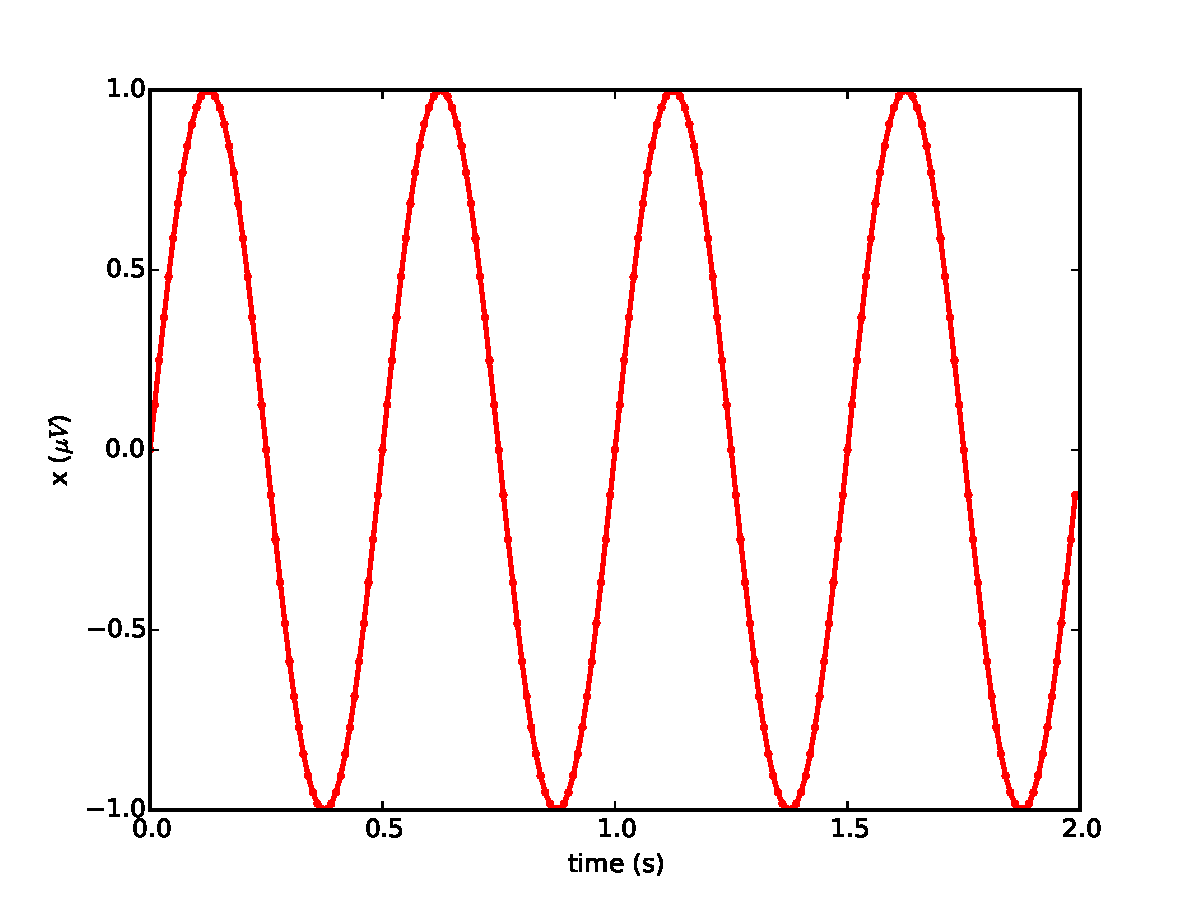
\includegraphics[width=5cm]{./fig/matplotlibSinus.pdf}
\end{minipage}
\end{frame}
%_______________________________________________________________________________


% import scipy.io
% mat = scipy.io.loadmat('file.mat')
%_______________________________________________________________________________
% 
% frame
%

\begin{frame}[fragile]
\frametitle{Numpy}
\framesubtitle{Tableaux ND et fonctions associ\'ees}

\begin{itemize}
 \item Les exemples sont donnés dans IPython avec les fonctions Pylab chargées.  
\end{itemize}

\begin{pythonConsole}
>>> A = array([[1,2,3],[4,5,6],[7,8,9]])
>>> whos

Variable   Type       Data/Info
-------------------------------
A          ndarray    3x3: 9 elems, type `int64`, 72 bytes

>>> A
array([[1, 2, 3],
       [4, 5, 6],
       [7, 8, 9]])
       
>>> A.size
9

>>> A.shape
(3,3)

>>> B = array([[1,0,0],[0,1,0],[0,0,1]])

>>> A*B

array([[ 1.,  0.,  0.],
       [ 0.,  5.,  0.],
       [ 0.,  0.,  9.]])
\end{pythonConsole}
\end{frame}

% 
% frame
% 

\begin{frame}
\frametitle{Numpy}
\framesubtitle{Tableaux ND et fonctions associ\'ees}
$\bullet$ M\'ethodes
\begin{itemize}
\item nonzero, max, min, mean, std ...
\item sum, cumprod, cumsum ...
\item reshape, resize, flatten, transpose ... 
\end{itemize}
\vspace{0.5cm}
$\bullet$ Fonctions
\begin{itemize}
\item $*$ : produit \'elt./\'elt.
\item $dot(.,.)$ : produit matriciel
\item ...
\end{itemize}
\end{frame}
%
% frame
%
\begin{frame}[fragile]
\frametitle{Numpy}
\framesubtitle{NDarray {\em vs.} matrix}
\begin{pythonConsole}
>>> A = array([[1.,2,3],[4,5,6],[7,8,9]])
>>> B = array([[1,0,0],[0,1,0],[0,0,1]])
>>> C = matrix([[1.,2,3],[4,5,6],[7,8,9]])
>>> D = matrix([[1,0,0],[0,1,0],[0,0,1]])

>>> whos
Variable   Type       Data/Info
-------------------------------
A          ndarray    3x3: 9 elems, type `float64`, 72 bytes
B          ndarray    3x3: 9 elems, type `int64`, 72 bytes
C          matrix     [[ 1.  2.  3.]\n [ 4.  5.  6.]\n [ 7.  8.  9.]]
D          matrix     [[1 0 0]\n [0 1 0]\n [0 0 1]]

>>> dot(A,B)

array([[ 1.,  2.,  3.],
       [ 4.,  5.,  6.],
       [ 7.,  8.,  9.]])

>>>  C*D

matrix([[ 1.,  2.,  3.],
        [ 4.,  5.,  6.],
        [ 7.,  8.,  9.]])

\end{pythonConsole}
\end{frame}

% 
% Slide
% 

\begin{frame}[fragile]
\frametitle{Numpy}
\framesubtitle{matrix}
$\bullet$ M\'ethodes
\begin{itemize}
\item min, max, mean, std, ...
\item .T, .H, .I, ...
\item reshape, flatten, ...
\end{itemize}
\vspace{0.2cm}
$\bullet$ Fonctions
\begin{itemize}
\item inv, svd, eig, ...
\end{itemize}
\vspace{0.2cm}
\underline{Diff\'erences entre array et matrix}
\begin{pythonConsole}
>>> A = array([[1.,2,3],[4,5,6],[7,8,9]])
>>> B = matrix([[1.,2,3],[4,5,6],[7,8,9]])

>>> A**2
array([[  1.,   4.,   9.],
       [ 16.,  25.,  36.],
       [ 49.,  64.,  81.]])

>>> B**2
matrix([[  30.,   36.,   42.],
        [  66.,   81.,   96.],
        [ 102.,  126.,  150.]])

\end{pythonConsole}
\end{frame}
%...............................................................................
%
% frame
%
%...............................................................................
\begin{frame}[fragile]
\frametitle{Numpy}
\framesubtitle{NDarray {\em vs.} matrix}
\begin{pythonConsole}
>>> A = array([[1.,2,3],[4,5,6],[7,8,9]])
>>> B = array([[1,0,0],[0,1,0],[0,0,1]])
>>> C = matrix([[1.,2,3],[4,5,6],[7,8,9]])
>>> D = matrix([[1,0,0],[0,1,0],[0,0,1]])

>>> whos
Variable   Type       Data/Info
-------------------------------
A          ndarray    3x3: 9 elems, type `float64`, 72 bytes
B          ndarray    3x3: 9 elems, type `int64`, 72 bytes
C          matrix     [[ 1.  2.  3.]\n [ 4.  5.  6.]\n [ 7.  8.  9.]]
D          matrix     [[1 0 0]\n [0 1 0]\n [0 0 1]]

>>> dot(A,B)

array([[ 1.,  2.,  3.],
       [ 4.,  5.,  6.],
       [ 7.,  8.,  9.]])

>>>  C*D

matrix([[ 1.,  2.,  3.],
        [ 4.,  5.,  6.],
        [ 7.,  8.,  9.]])

\end{pythonConsole}
\end{frame}
%...............................................................................
%
% frame
%
%...............................................................................
\begin{frame}[fragile]
\frametitle{Numpy}
\framesubtitle{matrix}
$\bullet$ M\'ethodes
\begin{itemize}
\item min, max, mean, std, ...
\item .T, .H, .I, ...
\item reshape, flatten, ...
\end{itemize}
\vspace{0.2cm}
$\bullet$ Fonctions
\begin{itemize}
\item inv, svd, eig, ...
\end{itemize}
\vspace{0.2cm}
\underline{Diff\'erences entre array et matrix}
\begin{pythonConsole}
>>> A = array([[1.,2,3],[4,5,6],[7,8,9]])
>>> B = matrix([[1.,2,3],[4,5,6],[7,8,9]])

>>> A**2
array([[  1.,   4.,   9.],
       [ 16.,  25.,  36.],
       [ 49.,  64.,  81.]])

>>> B**2
matrix([[  30.,   36.,   42.],
        [  66.,   81.,   96.],
        [ 102.,  126.,  150.]])

\end{pythonConsole}
\end{frame}
%...............................................................................
%_______________________________________________________________________________
%_______________________________________________________________________________
\subsection{Matplotlib}
%...............................................................................
\begin{frame}[fragile]
\frametitle{Matplotlib}
\framesubtitle{Librairie graphique}
\begin{itemize}
\item Outils graphiques 2D
\item Toolkits : Basemap, Axesgrid, mplot3d
\item Beaucoup d'exemples : www.matplotlib.org
\end{itemize}
\begin{minipage}{0.68\linewidth}
\begin{pythonConsole}
>>> t=arange(0,1,10e-5)
>>> S1=sin(2*pi*2*t);S2=sin(2*pi*7*t+(3*pi/7)),
>>> fig=figure()
>>> ax=fig.add_subplot(111,xlim=(-1,1),ylim=(-1,1))
>>> courbe=ax.plot(S1,S2);ax.grid('on')
>>> annotate('Courbe',xy=(-0.5,0.5),xytext=(-0.65,0),\
       bbox=dict(boxstyle='round,pad=0.5',fc='red',\ 
       alpha=0.2),arrowprops=dict(arrowstyle='->',\
         connectionstyle='arc3,rad=0'))
>>> title(r"Figure de Lissajous ($\nu_1=2$, $\nu_2=1$,\
         $\phi=\frac{3\pi}{7}$)")
>>> xlabel(r"$\sin(2\pi\nu_1 t)$")
>>> ylabel(r"$\sin(2\pi\nu_2 t + \phi)$")
>>> show()

\end{pythonConsole}
\end{minipage}
\begin{minipage}{0.3\linewidth}
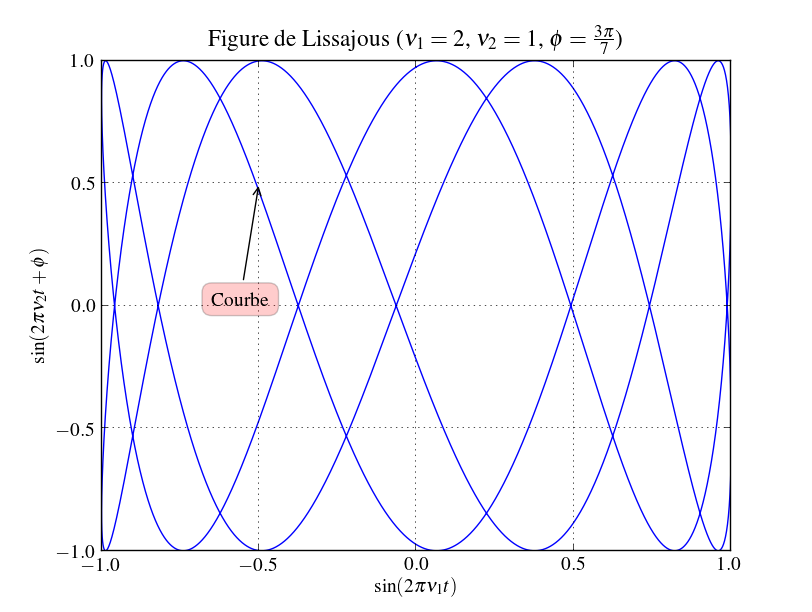
\includegraphics[width=4.5cm,height=4.5cm]{fig/Lissajous.png}
\end{minipage}
\end{frame}

% 
% Slide
% 

\begin{frame}[fragile]
\frametitle{Matplotlib}
\framesubtitle{Exemples}
\begin{minipage}{0.58\linewidth}
\begin{pythonConsole}
>>> [X,Y] = meshgrid(linspace(-2,2,500),\
linspace(-2,2,500))
>>> Z=X+Y*1j
>>> k=1
>>> while k<=75:
>>> 	Z = Z - (Z/3 - 1) / (3*Z**2)
>>>	k=k+1
>>> close('all')	
>>> imshow(angle(Z),cmap=cm.gray)
>>> #savefig('/MonChemin/Lenom.pdf',format='pdf')
>>> show()
\end{pythonConsole}
\end{minipage}
%\hspace{0.5cm}
\begin{minipage}{0.4\linewidth}
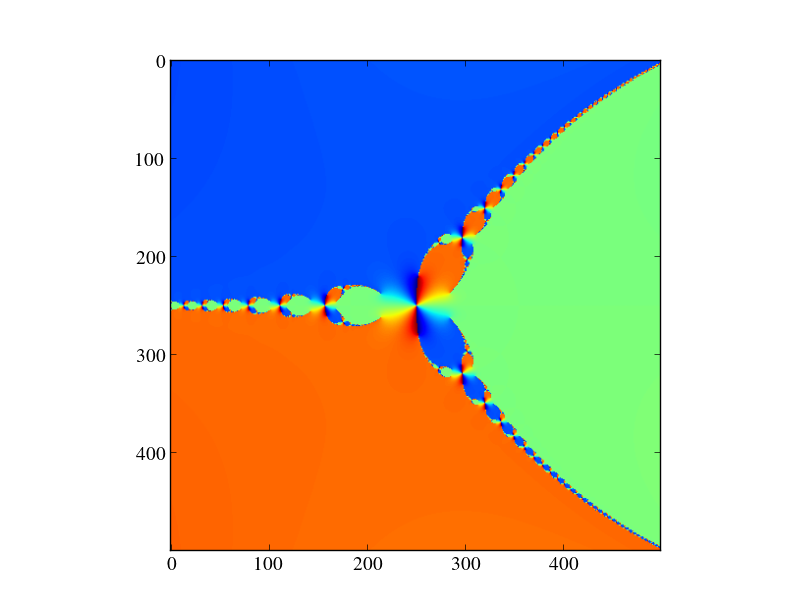
\includegraphics[width=5.5cm,height=4.5cm]{fig/fractal.png}
\end{minipage}
\end{frame}

% 
% Slide
% 
\begin{frame}
\frametitle{Matplotlib}
\framesubtitle{Exemples}

\begin{minipage}{0.4\linewidth}
\begin{figure}
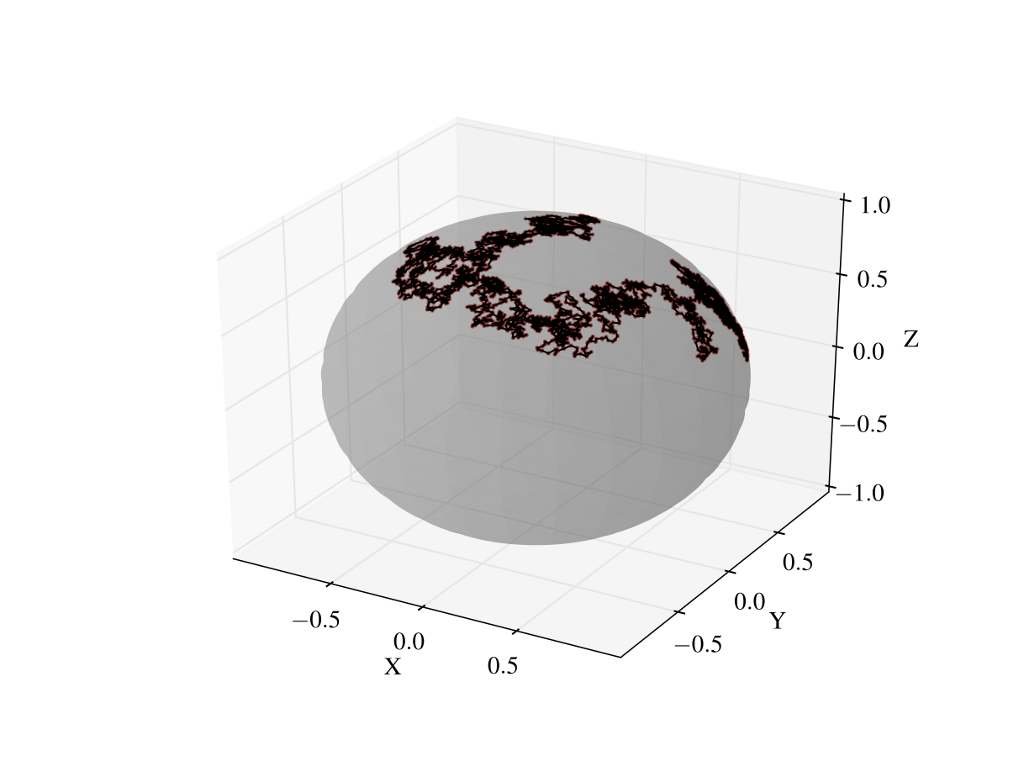
\includegraphics[width=6.5cm,height=5.5cm]{fig/BrownSphere.png}
\end{figure}
\end{minipage}
\hspace{1cm}
\begin{minipage}{0.4\linewidth}
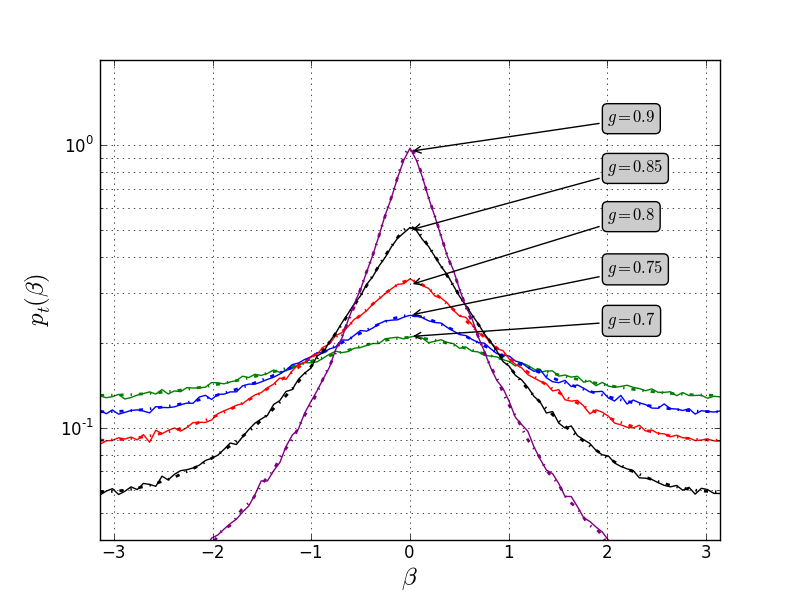
\includegraphics[width=5.5cm,height=4.5cm]{fig/Distrib.png}
\end{minipage}
\end{frame}
%...............................................................................
%_______________________________________________________________________________
%_______________________________________________________________________________
\subsection{Pylab}
%...............................................................................
\begin{frame}[fragile]
\frametitle{Pylab}
\framesubtitle{}
\begin{itemize}
 \item Module de Matplotlib : matplotlib\slash{}pylab.py
 \item Redéfinit des fonctions à la Matlab.
 \item Raccourci : "import pylab" au lieu de "import matplotlib.pylab"
 \item En général, et exceptionnellement, s'utilise : "from pylab import *" 
\end{itemize}
\begin{pythonConsole}
>>> from pylab import *
>>> plot([1, 5, 2, 4, 3])
[<matplotlib.lines.Line2D object at 0x4ec05b0>]
>>> show()
>>> a = randn(100, 10)
>>> type(a)
<type 'numpy.ndarray'>
>>> a.shape
(100, 10)
>>> help(matplotlib.pylab)
\end{pythonConsole}
\end{frame}
%...............................................................................
%_______________________________________________________________________________
%_______________________________________________________________________________
\subsection{Scipy}
%...............................................................................
\begin{frame}
\frametitle{Scipy}
\framesubtitle{Scientific library}
\begin{itemize}
 \item \myFig{height=0.5cm}{./fig/scipy-logo.png}\ : http://www.scipy.org 
\end{itemize}
\begin{center}
\tiny
\begin{tabular}{p{3cm}p{2cm}|p{3cm}p{2cm}}
Clustering package & scipy.cluster & Constants & scipy.constants \\
Discrete Fourier transforms & scipy.fftpack & Integration and ODEs & scipy.integrate \\
Interpolation & scipy.interpolate & Input and output & scipy.io \\
Linear algebra & scipy.linalg & Miscellaneous routines & scipy.misc \\
Multi-dimensional image processing & scipy.ndimage & Orthogonal distance regression & scipy.odr \\
Optimization and root finding & scipy.optimize & {\bfseries Signal processing} & scipy.signal \\
Sparse matrices & scipy.sparse & Sparse linear algebra & scipy.sparse.linalg \\
Compressed Sparse Graph Routines & scipy.sparse.csgraph & Spatial algorithms and data structures & scipy.spatial \\
Special functions & scipy.special & Statistical functions & scipy.stats \\
Statistical functions for masked arrays & scipy.stats.mstats & 
C/C++ integration & scipy.weave \\
\end{tabular}
\end{center}
\end{frame}
%...............................................................................
%_______________________________________________________________________________
%_______________________________________________________________________________
\subsection{Mayavi}
%...............................................................................
\begin{frame}
\frametitle{Mayavi}
\framesubtitle{}
\frameCC{%
\begin{itemize}
 \item Manipulation des objets 3D améliorée. 
\end{itemize}
}
{\myFig{width=9cm}{./fig/Mayavi.png}}
\end{frame}
%...............................................................................
%...............................................................................
\begin{frame}[fragile]
\frametitle{Mayavi}
\framesubtitle{import mayavi.engine}
\begin{itemize}
 \item Dans une console Python : import mayavi. \dots
\end{itemize}
\begin{pythonConsole}
>>> from numpy import array
>>> from mayavi.api import Engine
>>> engine = Engine()
>>> engine.start()
>>> engine.new_scene()
>>> from mayavi.sources.parametric_surface import ParametricSurface
>>> parametric_surface1 = ParametricSurface()
>>> scene = engine.scenes[0]
>>> engine.add_source(parametric_surface1, scene)
>>> from mayavi.modules.surface import Surface
>>> surface1 = Surface()
>>> engine.add_filter(surface1,parametric_surface1)
\end{pythonConsole}
\end{frame}
%...............................................................................
%_______________________________________________________________________________
%_______________________________________________________________________________
\subsection{Autres ressources : exemple C}
%...............................................................................
\begin{frame}[fragile]
\frametitle{Importation de bibliothèques de fonction écrites en C}
\framesubtitle{Exemple using module ctypes}
\begin{python}
import ctypes

myLib = ctypes.LoadLibray('myLib.lib')
fun_c = myLib.fun 
fun_c.argtypes = [ctypes.c_double, ctypes.c_int]
fun_c.restype = ctypes.c_int (default)

n = len(s)
pathFile = os.path.dirname(__file__)
libName = os.path.join(pathFile, 'clz.lib')
print('libName + ' + libName)
libCLZ = ctypes.CDLL(libName)
clz_c = libCLZ.clz
clz_c.restype = ctypes.c_uint
sequence = numpy.ctypeslib.ndpointer(dtype=numpy.int) 
clz_c.argtypes = ([sequence, ctypes.c_uint])
# conversion of s into sequence with numpy.asarray
c = clz_c(numpy.asarray(s, dtype='int'), n)
\end{python}
\end{frame}
%...............................................................................
\hide{%
%...............................................................................
\begin{frame}
\frametitle{Cython}
pas vu \dots
\end{frame}
%...............................................................................
}
\hide{%
%...............................................................................
\begin{frame}
\frametitle{Fortran to Python}
\framesubtitle{f2p}
Gestion des modules fortran cf Lapack 'f2p'. 

Importation comme les fonctions python import a.fun. 

En cours d'évaluation. 
\end{frame}
%...............................................................................
}
%_______________________________________________________________________________
%===============================================================================

%%% Local Variables: 
%%% mode: latex
%%% TeX-master: "presentationPython"
%%% End: 

%===============================================================================
\section{Distributions et Environnements de travail}
%===============================================================================
%_______________________________________________________________________________
\subsection{Python Software Foundation}
%...............................................................................
\begin{frame}
\frametitle{Python.org}
\framesubtitle{Official}
\frameCC{%
\begin{itemize}
 \item Python 2.7 ou 3.x téléchargeable sur \urlPython.
 \item Livré uniquemenent avec la bibliothèque standard. 
 \item Inclus l'interpréteur Python natif accessible à partir de l'environnement système. 
 \item Parfait pour tester des petits bouts de codes. 
\end{itemize}
}%
{\myFig{width=7cm}{./fig/interpreter.png}}
\end{frame}
%...............................................................................
%...............................................................................
\begin{frame}
\frametitle{Python IDLE}
\framesubtitle{official}
\frameCC{%
\begin{itemize}
 \item Python livré avec un Integrated DeveLopment Environment (IDLE) : 
 \begin{itemize}
 \footnotesize
  \item Une console Python : coloration automatique, autocomplétion \dots 
  \item Un éditeur de texte : indentation automatique, coloration syntaxique, debuggueur, \dots
 \end{itemize}
\end{itemize}
}%
{\myFig{width=8cm}{./fig/Idle.png}}
\end{frame}
%...............................................................................
%_______________________________________________________________________________
%_______________________________________________________________________________
\subsection{IPython}
%...............................................................................
\begin{frame}
\frametitle{IPython}
\framesubtitle{Intro}
\frameCC{%
\begin{itemize}
 \item \myFig{height=0.5cm}{./fig/IPy_header.png}\ IPy: \url{http://ipython.org}
 \item Console interactive accessible via le shell : coloration syntaxique, fonctions magiques, mémorisation des commandes, débuggueur, profileur, calculs parallèles \dots  
 \item Plusieurs options cf. 'man ipython' ou 'ipython -help'. 
\end{itemize}}
{\myFig{width=7cm}{./fig/IPython.png}}
\end{frame}
%...............................................................................
%...............................................................................
\begin{frame}
\frametitle{IPython}
\framesubtitle{Qtconsole}
\frameCC{%
\begin{itemize}
 \item Commande dans le shell : ipython qtconsole  
 \item Environnement graphique Qt qui permet de tracer des figures via matplotlib ou pylab.
 \item Commande directe : ipython qtconsole --pylab
\end{itemize}}
{\myFig{width=9cm}{./fig/IPythonQTConsole.png}}
\end{frame}
%...............................................................................
%...............................................................................
\begin{frame}
\frametitle{IPython}
\framesubtitle{notebook}
\frameCC{%
\begin{itemize}
 \small
 \item Commande dans le shell : ipython notebook  
 \item Editeur dans le navigateur HTML, \emph{Web-based interactive computational environment}. 
\end{itemize}}
{\myFig{width=9.5cm}{./fig/IPythonNotebook.png}}
\end{frame}
%...............................................................................
%...............................................................................
\begin{frame}
\frametitle{IPython}
\framesubtitle{notebook}
\frameCC{%
\begin{itemize}
 \small
 \item Cellules de codes ou de documentation : \emph{Cell Mode} à la Matlab, \emph{Document-Based Workflow} à la Mathematica. 
 \item Balisage du texte en LaTeX, HTML ou Markdown. 
\end{itemize}}
{\myFig{width=9.5cm}{./fig/IPythonNotebook.png}}
\end{frame}
%...............................................................................
%...............................................................................
\begin{frame}
\frametitle{IPython}
\framesubtitle{notebook}
\frameCC{%
\begin{itemize}
 \item Commande pour importer pylab et graphique dans l'interface html : 'ipython notebook --pylab inline'
 \item Génération de rapports dans le menu 'notebook > action > print' puis impression en pdf pour le navigateur HTML. 
\end{itemize}}
{\myFig{width=8cm}{./fig/IPythonNotebookInline.png}}
\end{frame}
%_______________________________________________________________________________
%_______________________________________________________________________________
\subsection{Enthought}
\begin{frame}
\frametitle{Enthought Canopy}
\begin{itemize}
 \item \myFig{height=0.5cm}{./fig/enthought-logo.png}\ : \url{https://www.enthought.com/products/canopy/}
 \item Contient Python et +100 librairies orientées applications scientifiques. 
 \item Multi-plateformes, \emph{Easy installation and update}.
 \item Gratuit pour les étudiants et les universitaires. 
 \item Anciennement Enthought Python Distribution EPD. 
 \item QtConsole, iPython. 
\end{itemize}
\end{frame}
%_______________________________________________________________________________
%_______________________________________________________________________________
\begin{frame}
\frametitle{Enthought Canopy}
\begin{center}
 \myFig{width=10cm}{./fig/enthought-canopy.jpg}
\end{center}
\end{frame}
%_______________________________________________________________________________
%_______________________________________________________________________________
\subsection{Python(x,y)}
%_______________________________________________________________________________
%_______________________________________________________________________________
\begin{frame}
\frametitle{Python(x,y)}
\frameCC{%
\begin{itemize}
\item \myFig{height=0.5cm}{./fig/PythonXYLogo.png}\ Python(x,y) : \url{https://code.google.com/p/pythonxy/}
\item \emph{\footnotesize Python(x,y) is a free scientific and engineering development software for numerical computations, data analysis and data visualization based on \emph{Python} programming language, \emph{Qt} graphical user interfaces and \emph{Spyder} interactive scientific development environment.}
\item Un grand nombre de librairies scientifiques, entre autres. 
\item Interface avec Eclipse (IDE principalement pour Java mais aussi Python). 
\end{itemize}
}
{\myFig{width=7cm}{./fig/pythonxy_home.png} \\ {\tiny source web}}
\end{frame}
%...............................................................................
%...............................................................................
\begin{frame}
\frametitle{Python(x,y)}
\framesubtitle{Spyder}
\frameCC{%
\begin{itemize}
\item Spyder (multiplateforme) : environnement de type Matlab pour Python. 
\end{itemize}
}
{\myFig{width=8cm}{./fig/Spyder.png} \\ {\tiny source web}}
\end{frame}
%_______________________________________________________________________________
\subsection{Anaconda}
%_______________________________________________________________________________
\begin{frame}
\frametitle{Anaconda}
\framesubtitle{}
\frameCC{%
\begin{itemize}
 \item \myFig{height=0.5cm}{./fig/continuum_analytics_logo.png} \, \url{http://continuum.io/downloads}
 \item \myFig{height=0.5cm}{./fig/anaconda_logo_web.png}
\end{itemize}
}
{%\myFig{width=8cm}{./fig/anaconda.png}
}
\end{frame}
%_______________________________________________________________________________
%_______________________________________________________________________________
\begin{frame}
\frametitle{Autres Integrated Development Environment}
\framesubtitle{}
\frameCC{%
\begin{itemize}
\item Tout éditeur de texte avec coloration syntaxique : Emacs, Vim, jEdit, gedit, Textpad... 
\end{itemize}
}
{\myFig{width=9cm}{./fig/jEdit.png}}
\end{frame}
%_______________________________________________________________________________
%_______________________________________________________________________________

%_______________________________________________________________________________
%_______________________________________________________________________________
%===============================================================================

%===============================================================================
\section{Conclusion}
%_______________________________________________________________________________
\subsection{Python vs Matlab ?}
%...............................................................................
\begin{frame}
\frametitle{Python vs Matlab}
\frameLR{6cm}{4cm}{%
\begin{itemize}
 \footnotesize
 \item Outils équivalents : matrices vs ndarray, console, script, graphisme, GUI, cell mode vs ipython notebook \dots
 \item Matlab, Matrix Laboratory, a des bibliothèques d'algèbre linéaire plus rapide que Numpy ou Scipy (sauf avec certaines distributions payantes). 
 \item Python est un langage de programmation.   
 \item Python est plus proche du code C pour prototyper.
 \item Chargement des modules à la volée en Python. 
 \item Python est gratuit. 
 \item Votre code en Python peut être utilisé gratuitement. 
\end{itemize}
}
{%
\myFig{width=4cm}{./fig/matlabLicenseManagerError4.png}
}
\end{frame}
%...............................................................................
%_______________________________________________________________________________

%===============================================================================


\frame{}
\appendix
\section{classe et variable 'self'}
%...............................................................................
\begin{frame}[fragile]
\frametitle{Classe exemples avec self}
\begin{itemize}
 \item Dans le corps de la classe, 'self' n'est pas défini. 
\end{itemize}
\begin{pythonConsole}
class Canard(): 
...     self.a = 10
... 
Traceback (most recent call last):
 File £"£<stdin>£"£, line 1, £in£ <module>
 File £"£<stdin>£"£, line 2, £in£ Canard
NameError: name £'self'£ £is not£ defined
\end{pythonConsole}
\end{frame}
%...............................................................................
%...............................................................................
\begin{frame}[fragile]
\frametitle{Classe exemples avec self}
\begin{itemize}
 \item Dans une méthode seul self.nomAttribut est accessible. 
\end{itemize}
\begin{pythonConsole}
class Canard(): 
...     a = 10
...     def __init__(self): 
...             self.b = 100
...             print(self.a)
...             print(b)
... 
riri = Canard()
10
Traceback (most recent call last):
 File £"£<stdin>£"£, line 1, £in£ <module>
 File £"£<stdin>£"£, line 6, £in£ __init__
NameError: £global£ name £'b'£ £is not£ defined
\end{pythonConsole}
\end{frame}
%...............................................................................
%...............................................................................
\begin{frame}[fragile]
\frametitle{Classe exemples avec self}
\begin{itemize}
 \item 'self' est conventionnel. 
 \item Le premier paramètre d'une méthode est considéré comme l'objet lui même. 
\end{itemize}
\begin{pythonConsole}
class Canard(): 
...     def __init__(obj): 
...             obj.a = 10
...             print(obj.a)
... 
riri = Canard()
10
\end{pythonConsole}
\end{frame}
%...............................................................................
%...............................................................................
\begin{frame}[fragile]
\frametitle{Classe exemples avec self}
\begin{itemize}
 \item Possibilité de rajouter des arguments optionnels lors de l'instanciation d'un objet. 
\end{itemize}
\begin{pythonConsole}
class Canard(): 
...     def __init__(self, patte=2):
...             self.a = patte
...             print(self.a)
... 
riri = Canard(patte=3)
3
\end{pythonConsole}
\end{frame}
%...............................................................................

%____________________________________________________________________________
\end{document}
%============================================================================

